%Examen 1,Extremos 
%Ejercicio 1
%Rojas Gutiérrez Rodolfo Emmanuel 
% Mestría en Probabilidad y Estadística.
\documentclass[10.5pt,notitlepage]{article}
\usepackage[utf8]{inputenc}
\usepackage{amsthm}
\usepackage{amsmath}
\usepackage{amsfonts}
\usepackage{mathtools}
\usepackage{amsmath,amssymb}       
\usepackage{enumitem}   
\usepackage{enumerate}
\usepackage{verbatim} 
\usepackage{bbm}
\usepackage[backend=biber,style=apa]{biblatex}
\usepackage{csquotes}
\DeclareLanguageMapping{spanish}{spanish-apa}
\urlstyle{same}
\addbibresource{refer.bib}
\usepackage{etoolbox}
\patchcmd{\thebibliography}{\section*{\refname}}{}{}{}
\usepackage{hyperref}
\usepackage{booktabs}
\renewcommand{\qedsymbol}{$\blacksquare$}
\usepackage{makecell}
\usepackage[spanish]{babel}
\decimalpoint
\usepackage[letterpaper]{geometry}
\usepackage{mathrsfs}
\newenvironment{solucion}
  {\begin{proof}[Solución]}
  {\end{proof}}
\pagestyle{plain}
\usepackage{pdflscape}
\usepackage[table, dvipsnames]{xcolor}
\usepackage{longtable}
\usepackage{tikz}
\def\checkmark{\tikz\fill[scale=0.4](0,.35) -- (.25,0) -- (1,.7) -- (.25,.15) -- cycle;} 
\usepackage[bottom]{footmisc}
\usepackage{hyperref}
\usepackage{float}
\usepackage[utf8]{inputenc}
\usepackage{placeins}
\DeclareMathOperator{\Tr}{Tr}
\DeclareMathOperator{\diag}{diag}
\newcommand{\PP}{\mathbb{P}}
\newcommand{\ZZ}{\mathbb{Z}}
\newcommand{\Bb}{\mathcal{B}}
\newcommand{\RR}{\mathbb{R}}
\newcommand{\Ff}{\mathcal{F}}
\newcommand{\FF}{\mathbb{F}}
\newcommand{\GG}{\mathbb{G}}
\newcommand{\Aa}{\mathcal{A}}
\newcommand{\Jj}{\mathcal{J}}
\newcommand{\Cc}{\mathcal{C}}
\newcommand{\oo}{\varnothing}
\newcommand{\ee}{\varepsilon}
\newcommand{\Ee}{\mathcal{E}}
\newcommand{\EE}{\mathbb{E}}
\newcommand{\NN}{\mathbb{N}}
\newcommand{\Pp}{\mathcal{P}}
\newcommand{\Ss}{\mathcal{S}}
\newcommand{\Mm}{\mathcal{M}}
\newcommand{\Hh}{\mathcal{H}}
\newcommand{\lL}{\mathrm{L}}
\newcommand{\Cov}{\mathrm{Cov}}
\newcommand{\Ll}{\mathcal{L}}
\newcommand{\xx}{\mathbf{x}}
\newcommand{\toPP}{\overset{\PP}{\to}}
\newcommand{\toCS}{\overset{\mathrm{c.s.}}{\to}}
\newcommand{\toL}{\overset{\mathrm{L}_1}{\to}}
\newcommand{\todis}{\overset{\mathrm{d}}{\to}}
\newcommand{\approxu}{\overset{u}{\approx}}
\newcommand{\igualD}{\overset{d}{=}}
\newcommand{\abs}[1]{\left\lvert #1 \right\rvert}
\newcommand{\norm}[1]{\left\| #1 \right\|}
\newcommand{\inner}[1]{\left\langle #1 \right\rangle}
\newcommand{\corch}[1]{\left[ #1 \right]}
\newcommand{\kis}[1]{\left\{ #1 \right\}}
\newcommand{\pare}[1]{\left( #1 \right)}
\newcommand{\floor}[1]{\lfloor #1 \rfloor}
\newcommand{\approxi}{\overset{i}{\approx}}
\newcommand{\Matrix}[1]{\begin{pmatrix} #1 \end{pmatrix}}

\theoremstyle{plain}

\newtheorem{thm}{Teorema}[section] % reset theorem numbering for each chapter
\newtheorem{defn}[thm]{Definición} % definition numbers are dependent on theorem numbers
\newtheorem{lem}[thm]{Lema} % same for example numbers
\newtheorem{remarkex}{Observación}
\newenvironment{rem}
  {\pushQED{\qed}\renewcommand{\qedsymbol}{$\triangle$}\remarkex}
  {\popQED\endremarkex}

\usepackage{geometry}
\usepackage{mathtools}
\usepackage{enumitem}
\usepackage{framed}
\usepackage{amsthm}
\usepackage{thmtools}
\usepackage{etoolbox}
\usepackage{fancybox}

\newenvironment{myleftbar}{%
\def\FrameCommand{\hspace{0.6em}\vrule width 2pt\hspace{0.6em}}%
\MakeFramed{\advance\hsize-\width \FrameRestore}}%
{\endMakeFramed}
\declaretheoremstyle[
spaceabove=6pt,
spacebelow=6pt
headfont=\normalfont\bfseries,
headpunct={} ,
headformat={\cornersize*{2pt}\ovalbox{\NAME~\NUMBER\ifstrequal{\NOTE}{}{\relax}{\NOTE}:}},
bodyfont=\normalfont,
]{exobreak}

\declaretheorem[style=exobreak, name=Ejercicio,%
postheadhook=\leavevmode\myleftbar, %
prefoothook = \endmyleftbar]{exo}
\usepackage{graphicx}
\graphicspath{ {images/} }
\title{Examen Parcial 2, Extremos \\
Ejercicio 1\\
Rojas Gutiérrez Rodolfo Emmanuel\\ 
Maestría en Probabilidad y Estadística.}
\date{\today}

\begin{document}
\maketitle
\setcounter{exo}{0}
\begin{exo}
 Considera la base de datos “sealevel2.csv” contiene diversos datos sobre el incremento en la altura del mar.
En particular, la columna 3 contiene información sobre el GMSL (Global Mean Sea Level, el cual se mide utilizando un satélite y considerando la diferencia entre una distancia dada por dicho satélite y la altura del mar). En la cuarta columna se encuentra la desviación estándar (STD) estimada del cambio entre cada medición. Con esta base de datos realiza lo indicado en cada uno de los siguientes puntos:
\begin{enumerate}
\item (5 pts.) Realiza la gráfica de dispersión de GMSL y STD y comenta lo observado.
\item (20 pts.) Estima el tiempo al cual el valor de GMSL estará nuevamente por encima de 50 y la STD volverá a ser superior a 100. Realiza esto usando excesos sobre un umbral y ajustando una DGVE. Comenta la validez de los resultados, elige una estimación y justifica el motivo de tu elección (deberás ser lo más formal posible).
\item (30 pts.) Estima el valor de GMSL y STD en el año 2025, condicionado al primer valor disponible en la base de datos.
\item (10 pts.) Estima la probabilidad de que la diferencia máxima entre dos valores consecutivos del GMSL exceda el máximo de tales diferencias reportado en los datos.
\item (10 pts.) Estima el valor esperado de la diferencia de dos valores consecutivos del GMSL, si se sabe que dicha diferencia ya ha sido mayor a 2.96.
\item (20 pts.) Repite los últimos dos incisos para los valores de la STD. 
\item (5 pts.) Compara y comenta lo observado en las gráficas de bondad de ajuste de cada punto, con lo observado en la gráfica de dispersión que presentaste en el punto 1.
\end{enumerate}
\end{exo}
\section{Soluciones.}
A modo de introducción, el conjunto de datos con el que se estará trabajando a lo largo de este examen, se presenta el en Cuadro \ref{tab:0}
\begin{table}[H]
        \centering
        \scalebox{0.8}{
        \begin{tabular}{@{}l@{\hskip 0.3in}r@{\hskip 0.3in}r@{}}
        \toprule
        Año&   \(GMSL\)&   \(STD\)\\
        \midrule          
  1993& -38.6&  89.9\\    
  1993& -42.0&  90.9\\    
  1993& -41.9&  87.3\\    
  \vdots&\vdots&\vdots\\
  2021&  49.6&  84.0\\     
  2021&  47.5&  82.7\\    
  2021&  50.1&  82.0\\     
        \end{tabular}}
        \caption{Datos del nivel global medio del mar, GMSL por sus siglas en ingles y, desviación estándar del cambio medido entre observaciones, abreviaba por sus siglas en inglés como \(STD\). Observaciones, hechas desde 1993 hasta 2021.}
        \label{tab:0}
\end{table}
El conjunto completo, puede consultarse en el script adjunto a este examen. Con esto en mente, se procederá a la solución de este ejercicio.

\subsection{Solución inciso 1.}
\begin{solucion}
En la Figura \ref{fig:1} puede observar los gráficos de dispersión solicitados. Primeramente, a su izquierda se puede observar el gráfico de dispersión de la variable \(GMLS\), dicha gráfica se hizo respetando el orden en el que las observaciones fueron reportadas, es decir, las observaciones que aparecen más hacia la izquierda son las más antiguas, mientras que, las observaciones hacia la derecha son las más recientes. De este modo, lo primero que resalta en este gráfico es, la tendencia creciente que presentan las observaciones \(GMLS\) con respecto al tiempo, lo que, es un patrón que no se espera en un conjunto de observaciones independientes provenientes de una misma distribución. Por otro lado, note que la variabilidad en las observaciones de \(GMLS\) parece ser constante, pues en cada zona del gráfico, si traza una linea vertical que cruce la nube de puntos, pareciera que los dos extremos en los que esta recta cortará a dicha nube, estarán siempre a la misma distancia sin importar a que altura del gráfico se trace la misma. Esta variabilidad, al menos de una medición de \(GMLS\) a la siguiente, ha sido estimada en la columna \(STD\) de la tabla de datos \ref{tab:0}. Ahora, a la derecha de la Figura \ref{fig:1}, puede observar una gráfica de dispersión de los datos en la columna \(STD\), siguiendo la misma idea que en la gráfica presentada para los datos de \(GMLS\), en cuanto al orden de gráficación. Note que, pese a que la variabilidad de \(GMLS\) medida por \(STD\) no es constante, la misma fluctúa de manera caso uniforme. Por otro lado, es importante mencionar que pese a que en esta gráfica no se percibe tendencia alguna, si parece presentar cierta periodicidad, pues, pueden observarse dos picos a lo largo del histórico en los que los valores de \(STD\) se disparan. 

Por lo comentado anteriormente, es claro, al menos en el caso de los datos \(GMLS\), que los datos de \(GMLS\) y \(STD\) no pueden ser independientes ni provenir de la misma distribución, no obstante, para la realización del inciso 2. se supondrá que esto es así, por lo que, bajo este contexto suponga que \(F\) es la distribución de los datos de \(GMLS\) y \(G\) la distribución de los datos en \(STD\). Entonces, dado que en la gráfica a la derecha de la Figura \ref{fig:1}, no parecen existir valores de \(GMLS\) muy separados de la nube de puntos, se concluye que bajo este criterio gráfico, no hay evidencia en contra de que la supuesta distribución común \(F\) de los mismos, posea extremo derecho finito. Por otro lado. para la distribución común \(G\) de los puntos en \(STD\), se tiene que bajo este criterio gráfico no existe evidencia en contra de que posea una cola pesada, por los dos picos presentados en la gráfica de dispersión a la izquierda de la Figura \ref{fig:1}, por lo que, al menos en esta primer prueba visual \(G\) pareciera poseer extremo derecho infinito. No obstante, este criterio gráfico es el menos relevante de todos, pues, es el que más depende en el criterio subjetivo del observador.      
\end{solucion}
\begin{rem}

A los largo de los análisis siguientes, el término cociente Fep empírico se empleara para hacer referencia, al cociente entre las Fep's empíricas de los diversos conjuntos de datos que serán analizados y la función identidad. Adicionalmente, la notación GPD\((\xi,a(u))\) será a abreviación utilizada para la Distribución Generalizada de Pareto con parámetros \(\xi\) de forma, \(a(u)\) de escala y \(0\) de localización. Finalmente, la notación DGVE\((\xi, a,b)\) denotara a la distribución Generalizada de Valores extremos con parámetros \(\xi\) de forma, \(a\) de escala y \(b\) de localización. 
\end{rem}

\subsection{Solución inciso 2.}
\begin{solucion}
Para este inciso, se comenzará analizando el conjunto de datos \(GMSL\), bajo el supuesto de que los mismos son independientes y provienen de la misma función de distribución \(F\). Para comenzar, en la Figura \ref{fig:2} puede observar una gráfica de la Fep empírica de estos datos, como puede ver la misma presenta una tendencia decreciente prácticamente uniforme, conforme crece el argumento donde esta es evaluada. De este modo, por la Proposición 2.5 de las notas de clase, se concluye que bajo este criterio gráfico no existe evidencia en contra de que la función de distribución \(F\) posea cola ligera, pues de poseer cola pesada, el único límite posible para la Fep asociada a \(F\), cuando el argumento donde es evaluada tiende al extremo derecho de \(F\), sería infinito, no obstante, en la gráfica comentada parece que de haber convergencia de la Fep empírica, cuando el argumento donde es evaluada tiende al extremo derecho de \(F\), dicha convergencia sería a lo más a un límite finito e inclusive cero.\footnote{Se sabe que, la Proposición citada solo esta enunciada si \(\omega_{F} = \infty\), no obstante, bajo el escenario en el que \(\omega_{F}< \infty\) es directo que \(F\) es de cola ligera, por lo cual, se sigue la conclusión de que bajo este criterio gráfico no hay evidencia en contra de este último hecho.}

Por otro lado, en la Figura \ref{fig:3} se deja una gráfica del cociente Fep empírico para los datos de \(GMSL\), además de una vista ampliada de los mismos, la cual va desde el cuantil muestral \(0.75\) hasta el cuantil muestral \(0.985\), lo que deja sin mostrar hacia la derecha, aquella parte de este cociente que es construida con a lo más el \(2\%\) de los datos hacia el extremo derecho de la distribución, evitando los picos que suelen formarse al final de este tipo de gráficos y que nublan el análisis de los mismos. Como puede ver, este cociente Fep empírico presenta una marcada tendencia decreciente, conforme crece el argumento en el que el mismo es evaluado, que parece culminar con una convergencia a cero, así, por la Proposición 2.7 y el Teorema 2.16 de las notas de clase, se concluye que bajo este criterio gráfico, no existe evidencia en contra de que \(F\) pertenezca al dominio de atracción Weibull o Gumbel.

Dado este último hecho, se decidió transformar los datos en \(GMSL\), que para fines de entendimiento denotaremos en este instante por \(\kis{x_1, \hdots, x_{1048}}\), de la siguiente manera:
\begin{equation}\label{lab.1}
y_i = \frac{1}{\max\kis{x_1, \hdots, x_{1048}} - x_i}, \text{ para  } i \in \kis{1, \hdots, 1048} \text{ tales que } x_i \neq  \max\kis{x_1, \hdots, x_{1048}},    
\end{equation}
pues, por el Teorema 2.10 de las notas de clase, si estos datos transformados no presentan evidencia en contra de su pertenencia al dominio de atracción Frechét, entonces, los datos originales de \(GMSL\) no presentan evidencia en contra de pertenecer al dominio de atracción Weibull.\footnote{En este caso, se usa el \(\max\kis{x_1, \hdots, x_{1048}}\) como una estimación del extremo derecho de \(F\), pues, aún no se determina que no existan evidencias en contra de la pertenencia de estos datos a algún dominio de atracción, por ende, esta es la mejor estimación de dicho extremo que se puede dar hasta este punto.} Cabe destacar que, a los datos transformados de \(GMSL\) mediante \eqref{lab.1}, se les denominará datos transformados de \(GMSL\). Ahora, en la Figura \ref{fig:4} se puede observar la gráfica de la Fep empírica para los datos transformados de \(GMSL\), además de una ampliación a la misma, que fue hecha desde el cuantil empírico de probabilidad \(0.65\), hasta el cuantil empírico de probabilidad \(0.985\) de los datos transformados de \(GMSL\). Como puede ver, esta gráfica presenta una tendencia creciente conforme el argumento en el que la misma es evaluada crece, a excepción de la parte en la que se forman bastantes picos hacia el final del gráfico, no obstante, la finalidad del zoom realizado es hacer notar que esto ocurre en las partes en las que la Fep se construyó con muy pocas observaciones. Por lo cual, de la Proposición 2.5 de las notas de clase, se concluye que bajo este criterio gráfico no hay evidencia en contra de que los datos transformados de \(GMSL\) posean una distribución de cola pesada. 

Por último, en la Figura \ref{fig:5} se deja una gráfica del cociente Fep empírico, para los datos transformados de \(GMSL\), además de un zoom a la misma realizado bajo el mismo criterio que el aplicado a la Fep empírica de estos datos, así, pese a que basados en la gráfica original de este cociente empírico, es complicado determinar un comportamiento de dicho cociente, conforme el argumento en el que se evalúa crece, si que es posible decir algo gracias al zoom realizado, pues, se puede apreciar que esta gráfica parece estabilizarse en un rango de valores entre \(2.5\) y \(3\), por lo que, parece existir convergencia de la misma hacia un valor en este intervalo. De este modo, por la Proposición 2.6 de las notas de clase, se concluye que bajo este criterio gráfico, no existe evidencia en contra de que la distribución de los datos transformados, pertenezca al dominio de atracción Frechét con \(\alpha >1\). Por lo que, no existe evidencia en contra de que la distribución \(F\) de los datos \(GMSL\), pertenezca al dominio de atracción Weibull. De este modo, por el Corolario 3.1 de las notas de clase, es posible aplicar método de exceso sobre un umbral para aproximar la cola de \(F\).

Para ello, primero se debe seleccionar un umbral adecuado para la aplicación del mismo. Para determinar dicho umbral, se empleo la función \(gpd.fitrange\) del paquete \(ismev\) de \(R\), con lo cual, se obtuvieron las primeras dos gráficas presentadas en la Figura \ref{fig:6}. Cabe destacar que, pese a que existe la recomendación empírica de seleccionar el parámetro de umbral para este ajuste, de tal suerte que la cola empírica de los datos evaluada en dicho umbral, se encuentre en el intervalo \([0.01, 0.05]\),  la función \(fit.range\) producía errores numéricos para los datos de \(GMLS\) si se deseaba elegir un umbral en esos niveles, por ende, se opto por elegir el umbral entre el cuantil empírico del \(0.94\) de probabilidad y, el cuantil empírico del \(0.95\) de probabilidad de estos datos.\footnote{Recuerde este criterio, pues, prácticamente fue empleado en cada elección de umbral de aquí en adelante.} Así, la primer gráfica en la Figura \ref{fig:6} corresponde a la estimación del parámetro de forma, de la GPD a ajustar a los datos de \(GMLS\) que exceden el umbral remarcado en el eje \(x\), donde, el eje \(x\) de dicha gráfica varia entre los cuantiles muéstrales mencionados. La segunda imagen, es una ampliación de la primera en el rango en el que se cree que esta última luce más estable, mirando fijamente esta segunda gráfica es fácil entender el porque se eligió un umbral de \(u_1 = 47.55\). Finalmente, habiendo seleccionado el umbral para el ajuste, se uso la función \(gpd.fit\) para llevar a cabo dicho ajuste y, con la función \(gpd.diag\) se produjeron las últimas dos gráficas en la Figura \ref{fig:6}, las cuales corresponden con un \(PP\) y una \(QQ\) del ajuste realizado. Como comentario final, los parámetros \(\xi_1\) y \(a_1\) de la GPD\((\xi_1,a_1)\) ajustada, pueden consultarse al pie de la Figura \ref{fig:6}, adicionalmente, con estos parámetros estimados\footnote{Se destaca, son parámetros estimados por método de máxima verosimilitud.} el ajuste parece razonable, pues, las gráficas \(PP\) y \(QQ\) presentadas, solo reflejan ligeras discrepancias hacia la parte central de la distribución. Por último, encuanto al ajuste del modelo respecta, cabe destacar que el parámetro estimado \(\xi_1\) es negativo, lo que va de acorde con el análisis hecho sobre \(F\) acerca de su posible posible pertenencia al dominio Weibull. 

Ahora, se proporcionaran tres formas para estimar los periodos de retorno solicitado: Las primeras dos corresponden al uso del método de excesos. Para iniciar, por el ajuste realizado se tiene que una primera y muy poco formal estimación, al periodo de retorno de \(GMSL\) a \(50\), en notación \(L_{F}(50)\), es: 
\begin{equation}\label{lab.app1}
L_{F}(50) = \frac{1}{\overline{F}(50)} = \frac{1}{\overline{F}(u_1 + 2.45)} \overset{i}{\approx}   \frac{1}{\overline{F}_{1048}(u_1)\overline{P}_{ \xi_1,a_1}(2.45)} = 22.914.     
\end{equation}
donde, \(\overline{F}_{1048}(u_1)\) denota a la función de distribución empírica de los datos \(GMSL\), evaluada en \(u_1\). Dicha idea, surge de que la aproximación:
\[
\overline{F}(50) \approx \overline{F}_{1048}(u_1)\overline{P}_{\xi_1,a_1}(2.45),
\]
si que esta justificada, por el Corolario 3.1 de las notas clase, la no evidencia en contra de la pertenencia de \(F\) al dominio Weibull y la Proposición 3.1 de las notas de clase. Así, el símbolo \(\approxi\) debe ser interpretado en este sentido intuitivo e informal. Para la segunda aproximación, se busca usar la relación existente entre los dominios Frechet y Weibull. Con esto en mente, dado que no existe evidencia en contra de que la distribución \(F\), de los datos de \(GMSL\), sea parte del dominio de atracción Weibull, es posible estimar el extremo derecho de la misma haciendo uso de la metodología vista en la ayudantía, así, puede ver que en la gráfica a la izquierda de la Figura \ref{fig:6.1}, una gráfica de la metodología vista en la ayudantía para la estimación del extremo derecho \(\omega_F\) de \(F\), en la cual puede observar que, para valores de entre \(25\) y \(50\) y valores entre \(200\) y \(250\), se observa cierta estabilidad en las estimaciones de \(\omega_F\), por ende, se decidió hacer uso de una valor que representará a estas dos conjuntos de puntos, en los que parece haber cierta estabilidad en el gráfico anterior. así, en linea roja se presenta una primera estimación para el extremo derecho \(\omega_{F}\), la cual se denotará por \(\hat{\omega}_{F}^{(1)}\) y posee un valor de \(64.909\), no obstante, al transformar los datos como se dirá a continuación, se llegaba a una contradicción con lo realizado hasta ahora. Se dedujo que esto puede deberse a que la estimación del extremo derecho, puede ser muy grande, pues, el máximo del conjunto de datos \(GMSL\) es \(57.92\), por lo que, la estimación final para \(\omega_{F}\) se obtuvo como el promedio de dicho máximo con \(\hat{\omega}_{F}^{(1)}\), a esta estimación, se le denotara como \(\hat{\omega}_{F}\) y posee un valor de \(61.414\). No es difícil convencerse, de que \(\hat{\omega}_{F}\) se encuentra un poco por encima, de la primer zona en la que se estabiliza el gráfico a la izquierda de la Figura \ref{fig:6.1}. Así, el efecto de haber hecho este promedio, es darle un mayor peso a la primer sección de la gráfica en la que hay estabilidad. 

Ahora, suponga que  \(\kis{x_1, \hdots ,x_{1048}}\) denota al conjunto de observaciones \(GMSL\), entonces, dichas observaciones son independientes y provienen de la distribución común \(F\), la cual no presenta evidencia en contra de su pertenencia al dominio de atracción Weibull. De este modo, el procedimiento para llevar a cabo la segunda estimación de \(L_{F}(50)\), consiste en:
\begin{itemize}
    \item[1.]  Se transforman los datos en \(\kis{x_1, \hdots ,x_{1048}}\) de la siguiente forma:
    \begin{equation}\label{trr}
         y_i = (\omega_{F} - x_i)^{-1}, \text{ para } i \in \kis{1, \hdots, 1048}.        
    \end{equation}
    \item[2.] Se ajusta una DGP a los datos transformados \(\kis{y_1, \hdots ,y_{1048}}\), los cuales, deberían de tener una distribución que no presente evidencias en contra de su pertenencia al dominio de atracción Frechét. Cabe destacar que, la forma en la que se llevo este paso en clase fue realizando el ajuste de una DGP, a los datos que pertenecen al dominio Weibull mediante el método de excesos sobre un umbral. Así, habiendo seleccionado un umbral para estos datos, el mismo se transforma de la siguiente manera \(u' = (\omega_{F} - u)^{-1}\). Finalmente, se hace uso de \(u'\) como el parámetro de umbral para ajustar la DGP a los datos \(\kis{y_1, \hdots ,y_n}\). Por ende, en este caso, el umbral \(u'\) sería \(u' = (\omega_{F} - u_1)^{-1}\).
    \item[3.] Sea \(\overline{P}_{\xi,a(u')}\) la cola de la distribución GPD\((\xi,a(u'))\) ajustada a los datos \(\kis{y_1, \hdots ,y_n}\), entonces, la aproximación del periodo de retorno \(L_{F}(50)\) de interés, puede hacerse de la siguiente manera
    \[
    L_{F}(50) = \frac{1}{\overline{F}(50)} = \frac{1}{\overline{F}_{*}((\omega_{F}- 50)^{-1 })} \approx \frac{1}{\overline{F}_{*}(u')\overline{P}_{\xi,a(u')}(x - u')} 
     \]
    donde, \(x = (\omega_{F}- 50)^{-1 } - u_1\), el signo \(\approx\) se debe interpretar como en la aproximación de la Proposición 3.3 de las notas de clase y, donde \(\overline{F}_{*}(x) = 1 - F(\omega_{F} - x^{-1})\mathbbm{1}_{\kis{x >0}}\) representa la cola de la distribución de los datos transformados. 
\end{itemize}
Ahora, el algoritmo anterior posee un gran problema: Se esta suponiendo que se conoce el extremo derecho de \(F\) y a \(\overline{F}^*\). No obstante, en clase se utilizo un estimador de \(\omega_{F}\), además de utilizar la cola empírica de los datos transformados para la estimación final. Así, una segunda estimación con un poco más de sustento teórico, puede darse como 
\[
 L_{F}(50) \overset{o}{\approx}  \frac{1}{\overline{F}_{n*}(u')\overline{P}_{\xi,a(u')}(x - u')} = 23.058,
\]
donde, \(\overline{F}_{n*}\) representa a la cola empírica, de los datos transformados de \(GMLS\) como en \eqref{trr}, usando \(\hat{\omega}_{F}\) en lugar de \(\omega_{F}\), mientras que, el signo \(\overset{o}{\approx}\) debe interpretarse en el sentido de la aproximación en el paso 3. del algoritmo mencionado. Por otro lado, el ajuste de la Pareto a los datos transformados puede verse en la Figura \ref{fig:7}, donde, también se presentan los parámetros estimados \(\xi\) y \(a(u')\). Cabe destacar que, el parámetro \(\xi\) para la GPD ajustada a los datos transformados es positivo, como era de esperarse. 

Por último, para ajustar una DGVE a los datos de \(GMSL\), observe que existen \(1048\) datos, que \(1048/8 = 131\) y que \(131\) es un número primo. De este modo, el tamaño máximo de bloques que se pueden formar de los \(1048\) datos de \(GMSL\), sin dejar ningún dato a fuera es \(8\). Se menciona esto, pues dado que los datos de \(GMSL\) no son observaciones de máximos, se debe obtener un conjunto de observaciones de este tipo, pues, dado que no hay evidencia en contra de que \(F\) este en el dominio Weibull, entonces, los máximos normalizados de variables independientes con distribución \(F\), se esperaría, converjan a una \(DGVE\) en distribución. Por otro lado, los bloques de los que se obtendrán los máximos se busca sean del tamaño más grande posible, pues, el resultado de convergencia mencionado es asintótico en el tamaño de los bloques. El procedimiento para calcular esto bloques, se describe a continuación: Los bloques se formaron eligiendo las primeras ocho observaciones en un bloque, luego las siguientes ocho en el siguiente bloque y así hasta acabar con todos las observaciones, de lo que se obtuvieron \(131\) bloques de diferencias, a los que se les calculo el máximo, lo que nos da un total de \(131\) observaciones de máximos de tamaño \(8\),  a lo cuales se le ajusto una DGVE con ayuda de la función \(gev.fit\), del paquete \(ismev\) de \(R\). Las gráficas de bondad y ajuste de este procedimiento, se obtuvieron con la función \(gev.diag\) y pueden verse en la Figura \ref{fig:7.1}, donde también se exponen los parámetros \(a\), \(b\) y \(\xi'\) estimados para el ajuste. Sobre la gráficas de bondad y ajuste, se comenta que la gráfica \(QQ\) presenta algunas discrepancias entre los datos y el modelo ajustado hacia la cola derecha de la distribución, al igual que hacia la cola izquierda. Adicionalmente, cabe destacar que en la gráfica \(PP\) también se resalta esta falta de ajuste, aunque de forma un poco menos marcada. No obstante, tomando en cuenta que el tamaño de bloque seleccionado para el cálculo de los datos de máximos de \(GMSL\) no es exageradamente grande, el ajuste presentado por las gráficas parece cuando menos razonable. Por último, en cuanto al ajuste respecta, es importante mencionar que el parámetro de forma \(\xi'\) estimado para este ajuste, es negativo lo que no contradice el análisis hecho sobre la posible pertenencia de \(F\) al dominio Weibull..

De este modo, dado el ajuste anterior es cuando menos razonable, entonces si \(H_{\xi',a,b}\) denota a la función de distribución de la \(DGVE\), ajustada a los máximos de \(GMLS\), se piensa que \(H_{\xi',a,b}\) es una aproximación razonable, a la distribución de máximos de \(8\) variables aleatorias independientes con distribución \(F\), pues, de esta distribución provienen los datos de  máximos a los que se les ajusto esta DGVEm bajo los supuestos planteados. Esto se menciona, pues, la tercer aproximación que se dará para \(L_{F}(50)\) es como sigue:\footnote{El superíndice \(mle\) hace referencia a que los parámetros usados para la DGVE ajustada, son estimaciones por máxima verosimilitud.} 
\[
L_{F}(50) = \frac{1}{\overline{F}(50)} = \frac{1}{1 - (F^{8}(50))^{1/8}} \overset{mle}{\approx} \frac{1}{1 - ({H_{\xi',a,b}(50))^{1/8}} }=  136.793.
\]
donde, dado que \(F^{8}\) es la función de distribución del máximo de \(8\) variables aleatorias independientes de distribución \(F\), se esta sustituyendo \(F^{8}\) por su aproximación con \(H_{\xi',a,b}\). De este modo, se deja en el Cuadro \ref{tab:1} las tres estimaciones obtenidas para \(L_{F}(50)\).
\begin{table}[H]
        \centering
        \begin{tabular}{@{}l@{\hskip 0.3in}r@{\hskip 0.3in}r@{\hskip 0.3in}r@{}}
        \toprule
         Valor de interés. & \(\approxi\) & \(\overset{o}{\approx}\) & \(\overset{mle}{\approx}\)\\
        \midrule         
        \(L_{F}(50)\)&22.914& 23.058 &136.793\\
        \end{tabular}
        \caption{Diversas aproximaciones para \(L_{F}(50)\).}
        \label{tab:1}
\end{table}
La elección, sobre que aproximación se elegiría, se presentará cuando también se tengan las aproximaciones correspondientes para \(STD\). Con esto en mente, se procederá al análisis de los datos de \(STD\), los cuales para fines de este inciso, se están suponiendo independientes y provenientes de la misma distribución \(G\). Así, para dar inicio a este análisis, puede observar en la Figura \ref{fig:8} una gráfica de la Fep empírica de estos datos. Observando dicha gráfica, note que en un inicio la misma presenta una tendencia decreciente, que cambia en el intervalo de \([85,93]\), para volver a adoptar una tendencia decreciente, mucho menos remarcada que en un principio, en el intervalo \([93,100]\). Ahora, se puede pensar que este cambio puede deberse al bajo número de exdencias existentes, no obstante, sobre el primer umbral de \(93\), marcado en este gráfica por la primer linea negra vertical, existen \(88\) observaciones de \(STD\), mientras que, sobre el segundo umbral marcado el cual posee un valor de \(100\) existen aún \(39\) observaciones de \(STD\), por lo cual, la sección del gráfico atrapada entre esta dos lineas verticales, fue construida con a lo menos \(39\) observaciones, por lo que, se piensa que esta cantidad es aún significativa para determinar el comportamiento de la gráfica anterior.\footnote{Al ver esto, fue que se eligió usar el cuantil muestral del \(0.985\) para realizar ZOOM's en este trabajo, pues, esto oculta hacia la derecha únicamente aquella parte del gráfico que esta hecha con a lo más el \(2\%\) de la muestra, i.e, a lo mas unas \(20\) observaciones.} 

De este modo, por la Proposición 2.5 de las notas de clase, se concluye bajo este criterio gráfico, que no existe evidencia en contra de que la función de distribución \(G\) posea cola ligera, pues de poseer cola pesada, el único límite posible para la Fep asociada a \(G\), cuando el argumento donde la misma es evaluada tiende al extremo derecho de \(G\), sería infinito, sin embargo, en la gráfica citada parece que de haber convergencia de la Fep empírica, cuando el argumento donde esta es evaluada tiende al extremo derecho de \(G\), dicha convergencia sería a lo más a un límite finito ó inclusive cero.

Por otra parte, en la Figura \ref{fig:9} se deja un gráfico del cociente Fep empírico para los datos de \(STD\), además de una vista ampliada de los mismos, la cual va desde el cuantil muestral \(0.75\) hasta el cuantil muestral \(0.985\). Como puede ver, este cociente Fep empírico preserva la forma final de la Fep para estos datos, presentando las mismas tendencias en el mismo orden, i.e, decreciente, creciente para finalizar en una tendencia decreciente. No obstante, es confuso el final de la gráfica, por un lado, si se ve la misma sin acercamiento, puede notarse que la tendencia decreciente continua y parece terminar con una convergencia a cero, pero, al acercarla se nota cierta estabilidad en un rango de valores, muy cercanos a cero pero aún positivos. Por ende, bajo este criterio gráfico es complicado obtener una conclusión, pues si bien, la gráfica sin acercamiento del cociente empírico mantiene la tendencia decreciente hasta acabar en cero, lo cual apunta a los dominios de atracción Weibull o Gumbel, no menos cierto es que la parte que no se muestra en el aumento, se ha construido con muy pocos datos. De este modo, para recabar más información se transformaran los datos de \(STD\), los cuales para fines de notación se denotarán en este instante por \(\kis{z_1, \hdots, z_{1048}}\), de la siguiente manera:
\begin{equation}\label{lab.1'}
y_i = \frac{1}{\max\kis{z_1, \hdots, z_{1048}} - z_i}, \text{ para  } i \in \kis{1, \hdots, 1048} \text{ tales que } z_i \neq  \max\kis{z_1, \hdots, z_{1048}},    
\end{equation}
pues, por el Teorema 2.10 de las notas de clase, si estos datos transformados no presentan evidencia en contra de su pertenencia al dominio de atracción Frechét, entonces, los datos originales de \(STD\) no presentan evidencia en contra de pertenecer al dominio de atracción Weibull. Se resalta que, se hará referencia a los datos transformados de \(STD\) mediante \eqref{lab.1'}, como datos transformados de \(STD\). Así, en la Figura \ref{fig:10} se puede observar la gráfica de la Fep empírica para los datos transformados de \(STD\), en conjunto con una ampliación de la misma, que fue hecha desde el cuantil empírico de probabilidad \(0.65\), hasta el cuantil empírico de probabilidad \(0.985\) de los datos transformados de \(STD\). Como puede ver, esta gráfica presenta una tendencia creciente bastante marcada, conforme el argumento en el que la misma es evaluada crece, a excepción de la parte en la que se forman bastantes picos hacia el final del gráfico, empero, la finalidad del zoom realizado es resaltar que esto ocurre en las partes en las que la Fep se construyó con muy pocas observaciones. Por lo cual, de la Proposición 2.5 de las notas de clase, se concluye que bajo este criterio gráfico no hay evidencia en contra de que los datos transformados de \(STD\) posean una distribución de cola pesada. 

Por otro lado, en la Figura \ref{fig:11} se deja una gráfica del cociente Fep empírico, para los datos transformados de \(STD\), junto a un zoom realizado a este bajo el mismo criterio que el aplicado a la Fep empírica de estos datos. De este modo, centre su atención en el zoom realizado, pues gracias a este se puede observar que conforme crece el argumento en el que este cociente es evaluado, el mismo presenta una tendencia creciente, que parece irse perdiendo hacia el final del gráfico, de hecho, cuando el cociente alcanza el valor de \(2.5\) el mismo parace estabilizarse a esa altura, esto se ve remarcado al observar la gráfica no ampliada del cociente \(Fep\) empírico, pues, cuando esta llega a la altura de \(2.5\) parece estabilizarse por un tiempo, para después formar los picos usuales por bajo número de excedencias. De esta manera, por la Proposición 2.6 de las notas de clase, no existe evidencia en contra de que la distribución de los datos transformados de \(STD\), pertenezca al dominio de atracción Frechét con \(\alpha >1\). Por lo que, no existe evidencia en contra de que la distribución \(G\) de los datos \(GMSL\), pertenezca al dominio de atracción Weibull. Así, por el Corolario 3.1 de las notas de clase, es posible aplicar método de exceso sobre un umbral para aproximar la cola de \(G\).

Con esto en mente, primero se debe seleccionar un umbral adecuado para la aplicación del método. Para esta tarea, se empleo la función \(gpd.fitrange\) de \(R\), con lo cual, se obtuvieron las primeras dos gráficas presentadas en la Figura \ref{fig:12}. Cabe destacar que, para preservar un criterio uniforme para la selección de umbrales a lo largo de este examen, se optó por elegir el mismo entre el cuantil empírico del \(0.94\) de probabilidad y, el cuantil empírico del \(0.95\) de probabilidad de estos datos. De este modo, la primer gráfica en la Figura \ref{fig:12} corresponde a la estimación del parámetro de forma, de la GPD a ajustar a los datos de \(STD\) que exceden el umbral remarcado en el eje \(x\), donde, el eje \(x\) de esta gráfica varia entre los cuantiles muéstrales mencionados. La segunda imagen, es una ampliación de la primera en el rango en el que se cree que esta última luce más estable, mirando fijamente esta segunda gráfica es fácil entender el porque se eligió un umbral de \(u_2 = 96.5\). Para finalizar, una vez seleccionado el umbral para el ajuste, se empleo la función \(gpd.fit\) para llevar a cabo dicho ajuste y, con la función \(gpd.diag\) se construyeron las últimas dos gráficas en la Figura \ref{fig:12}, las cuales corresponden con un \(PP\) y una \(QQ\) del ajuste realizado. Como comentario final, los parámetros \(\xi_2\) y \(a_2\) de la GPD\((\xi_2,a_2)\) ajustada, pueden consultarse al pie de la Figura \ref{fig:12}, adicionalmente, con estos parámetros estimados el ajuste parece razonbles, pues, las gráfica \(PP\) presentada solo refleja ligeras discrepancias hacia la parte central de la distribución, mientras que, la respectiva gráfica \(QQ\) solo presenta discrepancias hacia la cola derecha de la misma, lo que es común en este tipo de gráficos. Por último, en cuanto al ajuste respecta, puede ver que el parámetro de forma estimado \(\xi_2\), es negativo lo cual actúa en favor del análisis realizado previamente sobre \(G\), respecto a su posible pertenencia al dominio Weibull.

Ahora, antes de pasar a las aproximaciones del periodo de retorno \(L_{G}(u)\) solicitado, es menester ajustar una DGVE a los máximos por año de \(STD\). Para ello, se calcularon dichos máximos y a este conjunto de \(29\) datos, se les ajusto una DGVE con ayuda de la función \(gev.fit\) del paquete \(ismev\) de \(R\). Las gráficas de bondad y ajuste de este procedimiento, fueron construidas empleando la función \(gev.diag\) y pueden verse en la Figura \ref{fig:14.1}, donde también se exponen los parámetros \(a\), \(b\) y \(\xi'\) estimados para el ajuste. Sobre la gráficas de bondad y ajuste, en la cual puede notar que el ajuste es bastante bueno, salvo por las discrepancias presentadas en la gráfica \(QQ\) hacía la cola de la distribución, no obstante, este comportamiento es de esperarse en este tipo de gráficos. Lo que si llama la atención, es que en este caso el parámetro de forma \(\xi'\) estimado sea positivo. No obstante, al igual que en el caso de los máximos en \(GMSL\), de los bloques con los se calcularon los \(131\) máximos con los que se llevo a cabo el ajuste, tienen una tamaño de \(m = 36\), por lo que, posiblemente el tamaño de muestra empleado para los bloques, no es suficientemente grande como para que se pueda aproximar la distribución de los mismos mediante una DGVE, esta hipótesis se tiene, pues si en el ajuste de la Pareto se elegía un umbral pequeño, también se estimaba un parámetro de forma positivo para la \(GPD\) ajustada. En adición, esto podría explicar porque la gráfica \(QQ\) de este ajuste, presenta un poco más de discrepancias hacia la cola derecha de la distribución, que la gráfica equivalente para los datos de \(GMSL\). no obstante, al final de este ejercicio se comentará un poco más sobre esto.

Finalmente, las aproximaciones que se presentaran a continuación, fueron obtenidas bajo las mismas ideas que las correspondientes aproximaciones para \(GMSl\), haciendo los cambios respectivos de \(\overline{F}\), \(\overline{F}_{1048}\), \(\overline{P}_{\xi_1,a_1}\), \(u_1 = 47.55\) \(H_{\xi,a,b}\), \(\hat{\omega}_F\)  y \(50\) por  \(\overline{G}\), \(\overline{G}_{1048}\), \(\overline{P}_{\xi_2,a_2}\), \(u_2 = 96.5\) \(S_{\xi',a,b}\) y \(100\), donde, \(\overline{G}_{1048}\) es la cola empírica de los datos de \(STD\), \(\overline{P}_{\xi_2,a_2}\) es la cola de la GPD\((\xi_2,a_2)\) a los datos de STD que exceden el umbral \(u_2\) y \(S_{\xi',a,b}\) es la función de distribución de la DGVE ajustada a los máximos de lo datos de \(STD\), los cuales se obtuvieron bajo la misma metodología que en el caso anterior. Cabe destacar que, para aproximar el extremo derecho \(\omega_{G}\) de  \(G\), se volvió a emplear la método vista en la ayudantía, la aplicación gráfica del mismo puede verse a la derecha de la Figura \ref{fig:6.1}, en esta se puede ver nuevamente dos regiones en las que la estimación de \(\omega_{G}\) parece estabilizarse, por lo que, para tomar un valor representativo entre estas dos regiones, se hizo uso del promedio de las estimaciones, el cual se denota en está gráfica por la linea roja horizontal trazada. El valor obtenido mediante este método, se denotará por \(\hat{\omega}_{G}\), es igual a \(120.593\) y se empleo en lugar de \(\hat{\omega}_{F}\), en los procedimientos realizados para obtener las siguientes estimaciones. Con esto en mente, las respectivas aproximaciones para \(L_{G}(100)\) se presentan en el Cuadro \ref{tab:2}
\begin{table}[H]
        \centering
        \begin{tabular}{@{}l@{\hskip 0.3in}r@{\hskip 0.3in}r@{\hskip 0.3in}r@{}}
        \toprule
         Valor de interés & \(\approxi\) & \(\overset{o}{\approx}\) & \(\overset{mle}{\approx}\)\\
        \midrule         
        \(L_{G}(100)\)&24.842& 26.618 &135.675\\
        \end{tabular}
        \caption{Diversas aproximaciones para \(L_{G}(100)\).}
        \label{tab:2}
\end{table} 
Es importante mencionar, que la aproximación \(\overset{o}{\approx}\) se realiza un ajuste GPD, a los datos transformados de \(STD\) como en\footnote{Evidentemente, haciendo los cambios correspondientes como quitar \(\hat{\omega}_{F}\) por \(\hat{\omega}_G\).} \eqref{trr}, el diagnóstico de este ajuste puede verse en la gráfica en la Figura \ref{fig:14}, esto se menciona para destacar dos cosas: La primera es que, el ajuste de esta \(GPD\) a los datos transformados de \(STD\) es bueno, pues, solo se presentan las típicas discrepancias en la \(QQ\) hacia la cola de la distribución, por otro lado, el parámetro de forma estimado para este ajuste es positivo, lo cual es consistente con el análisis hecho sobre \(G\) y su posible pertenencia al dominio Weibull. 


Finalmente, viendo los valores reportados en los Cuadros \ref{tab:1} y \ref{tab:2}, es claro que existen grandes discrepancias entre los métodos que ocupan el método de excesos, y aquellas aproximaciones que hacen uso del ajuste de una DGVE, sin embargo, en el caso de los datos en \(STD\) me quedaría con la aproximación del periodo de retorno proporcionada, por el método de excesos por la cuestión de que el parámetro de forma estimado para el ajuste de la \(DGVE\) a los máximos de \(STD\), no resultaba consistente con el análisis previamente hecho, ni con el análisis que se presentará al final de este ejercicio. No obstante, en el caso de los datos \(GMSL\) me quedaría con ambas, y se preguntará ¿por qué? Para explicar esta elección, observe nuevamente el gráfico de dispersión de estos datos, gráfica a la izquierda de la Figura \ref{fig:1} y, note como a lo largo de los \(1048\) periodos que comprenden los años de observación, solo se esta por encima de \(50\) en periodos mayores a \(800\), de hecho el primer periodo en el que \(GMSL\) rebasa el valor de \(50\) es en el periodo \(1007\). No obstante, después de dicho periodo, el valor de \(GMSL\)  esta por encima de \(50\) prácticamente en todos los casos, por lo que, el retorno es inmediato a partir de este momento. Este razonamiento puede explicar el porque, el periodo de retorno estimado de una forma sale muy pequeño mientras el otro es bastante grande. No obstante, sin llevar a cabo este razonamiento, para mi la estimación mas fiable es la denotada por \(\overset{o}{\approx}\), pues, la misma es la que posee un poco mas de sustento teórico.  Con esto, se concluye el segundo númeral de esta tarea. 

\begin{rem}
Como observación final, dado que en el análisis de los datos en \(STD\) se llego en cierta forma a una contradicción, pues, la estimación del parámetro de forma de la DGVE ajustada a los máximos de \(STD\) es positiva, se llevaron a cabo las pruebas \(G_{n,k}(0)\) vistas en la ayudantía. Dichas pruebas, pueden hacerse pues no existe evidencia en contra de que \(G \in D(H_{\xi})\) para alguna \(\xi \in \RR\), la cual dados lo análisis previos, no tiene evidencia en contra de ser negativa. 

De este modo, en la Figura \ref{fig:15}, se presenta a su izquierda una gráfica de los \(p\)-valores de la prueba de hipótesis \(\mathcal{H}_0: \xi = 0\) vs \(\mathcal{H}_1: \xi < 0\), mientras que, de lado derecho se presenta el contraste \(\mathcal{H}_0: \xi = 0\) vs \(\mathcal{H}_1: \xi > 0\). En ambas gráficas, se ha trazado una recta horizontal de color rojo situada a la altura \(0.05\). Como puede ver, en general no es posible rechazar bajo un nivel de significancia del \(5\%\), la hipótesis nula cuando la hipótesis alternativa es \(\mathcal{H}_1: \xi >0\), empero, es posible rechazar para diversas elecciones de \(k_{n}\) la hipótesis nula cuando la hipótesis alternativa es \(\mathcal{H}_1: \xi < 0\). Adicionalmente, para valores de \(k_{n}\) mayores a \(\floor{n^{0.6}}\) con \(n = 1048\), se observo que las gráficas de los \(p\)-valores parecen variar de forma irregular, por lo que, se decidió tomar este valor de corte. Esto, refuerza el hecho de que no hay evidencia en contra de que \(\xi <0\), i.e, que no hay evidencia en contra de que \(G\) pertenezca al dominio Weibull. 

\end{rem}
\end{solucion}
\newpage
Para lo que resta de este ejercicio, será necesario definir los datos de diferencias entre dos observaciones consecutivas, tanto de \(STD\) como de \(GMSL\). Primeramente, denote los datos observados de \(GMSL\) como \(\kis{x_1, \hdots, x_{1048}}\), donde la enumeración se ha asignado de acuerdo al orden de ocurrencia de los mismos de manera ascendente, esto quiere decir que, el dato etiquetado con el número \(1\) es el primer dato observado de \(GMSL\), i.e. el primer dato en la columna \(GMLS\) en el Cuadro \ref{tab:0}, mientras que, el dato indexado con el número \(1048\), es la última observación realizada sobre la variable \(GMSL\). De este modo, el conjunto \(\kis{w_1, \hdots,w_{1048}}\) de datos de diferencias entre dos valores consecutivos de \(GMSL\), al cual a se hará referencia a partir de este punto como datos de \(diffGMLS\), está dado por:
\begin{align*}
 w_1 = x_1 \text{ y } w_{i} = x_{i} -x_{i-1} \text{ para } i \in \kis{2, \hdots, 1048}.  
\end{align*}
Por otro lado, denote los datos observados de \(STD\) como \(\kis{z_1, \hdots, z_{1048}}\), donde la enumeración se ha asignado de acuerdo al orden de ocurrencia de los mismos de manera ascendente. Entonces, el conjunto \(\kis{s_1, \hdots,s_{1048}}\) de datos de diferencias entre dos valores consecutivos de \(STD\), al cual a se hará referencia a partir de este punto como datos de \(diffSTD\), está dado por:
\begin{align*}
 s_1 = z_1 \text{ y } s_{i} = z_{i} -z_{i-1} \text{ para } i \in \kis{2, \hdots, 1048}.  
\end{align*}
Ahora, se hará un análisis similar sobre pertenencia de estos datos a algún dominio de atracción. Con esto en mente, se iniciará analizando el conjunto de datos de \(diffGMLS\). Así, en la Figura \ref{fig:17} puede ver un gráfico de dispersión de las datos de \(diffGMLS\), dicha gráfica se hizo respetando el orden impuesto en el conjunto de observaciones enumerado \(\kis{w_1, \hdots, w_{1048}}\). De este modo, lo primero que resalta en este gráfico es que no parece existir ni estacionariedad, ni tendencia en la nube de puntos formada por estos datos, en realidad dichos datos parecen estar acomodados de manera aleatoria al rededor de cero, más aún, salvo el valor extremo que se ve hacia el extremo izquierdo de la distribución, el cual es precisamente \(w_{1} = -38.59\),\footnote{Lo cual tiene sentido, pues en si esta primer observación no es una diferencia.} parece razonable pensar que todos estos datos provienen de una misma distribución, pues, casi todos los valores observados se encuentran en la misma franja de valores de \(10\) a \(-10\) y, la distribución de los mismos a lo largo de dicha franja es muy similar. Esto se comenta, pues a partir de este punto y para fines de aplicación de los métodos vistos hasta ahora en clase, será necesario suponer a lo largo de lo que resta de esta examen, que los datos de \(diffGMLS\) son observaciones independientes y con una misma distribución \(F^{(1)}\), y por las razones expuestas este supuesto no es tan descabellado, al menos no tanto como en los primero conjuntos de datos. Adicionalmente, se supondrá que dicha distribución \(F^{(1)}\) es continua, lo cual tiene sentido, por todos los valores posibles que pueden tomar estas diferencias consecutivas, entre valores del nivel del mar el cual es una variable aleatoria continua. 


Con esto en mente, se procederá a ver si existe o no evidencia en contra de la pertenencia de \(F^{(1)}\), a algún dominio de atracción maximal. Para ello, vuelva a fijar su atención en la Figura \reg{fig:17} y, observe que existen unas cuantas observaciones en este gráfico de dispersión, que se alejan de la nube de puntos en dirección hacia arriba de la misma, por lo cual, bajo este criterio gráfico parece ser que \(F^{(1)}\) posee cola pesada, no obstante, tenga en cuenta que este es un criterio muy subjetivo. 

Ahora, se deja en en lado izquierdo de la Figura \ref{fig:17.1},  una gráfica de la Fep empírica de estos datos, como puede ver, la Fep empírica presenta una tendencia decreciente conforme crece el argumento donde esta es evaluada, dicha tendencia se mantiene hasta el punto \(x = 5\), el cual se encuentra marcado en esta gráfica por una linea recta horizontal. En primera instancia, uno podría creer que este efecto, se debe a que existe un pobre número de observaciones de \(difGMLS\) que exceden al número \(5\), no obstante, existen \(29\) datos de diferencias que exceden este umbral lo cual no es mucho, pero tampoco es una cantidad despreciable. Más aún, si se hace un aumento en esta gráfica, bajo el criterio empleado a lo largo de este examen, es decir, se hace un zoom de esta gráfica para valores que se encuentran entre el cuantil muestral de probabilidad \(0.65\) y, el cuantil muestral de probabilidad \(0.985\) de los datos de \(diffGMLS\), ver gráfica a la derecha de la Figura \ref{fig:17.1}, uno puede notar, como esta gráfica después de decrecer un tiempo comienza a crecer de manera acelerada. Por ende, pese a que en un principio se pensaría que esta Gráfica, junto con la Proposición 2.5 de las notas de clase, apuntan a que no existe evidencia en contra de que la función de distribución \(F^{(1)}\) posea cola ligera, puede que este comportamiento, primeramente decreciente y posteriormente creciente de la Fep empírica, sea similar al ejemplo Pareto visto en la clase previa al examen, en el que la Fep asociada a la Pareto empleada, después de decrecer de manera continua en un intervalo considerable de valores, comenzaba a crecer poco a poco. Por ende, este criterio gráfico parece no aportar demasiada información sobre \(F^{(1)}\).   

Ahora, en la Figura \ref{fig:18} se deja una gráfica del cociente Fep empírico para los datos de \(diffGMSL\), además de una vista ampliada de los mismos, la cual va desde el cuantil muestral de probabilidad \(0.65\), hasta el cuantil muestral de probabilidad \(0.985\). Note que, pese a que en la gráfica original de este cociente Fep empírico, pareciera que el mismo tiende a cero conforme crece el argumento en el que el este es evaluado, dicho efecto es engañoso, por la escala en la que se presenta el eje \(y\) de esta gráfica. Esto último, se corrobora al observar la vista ampliada de la misma, pues, como puede ver este cociente esta aún bastante lejos de llegar al cero. Más aún, en la vista ampliada presentada, se nota como la tendencia decreciente de este cociente, parece irse alentando y estabilizarse en un valor mayor a cero. De esta manera, por la Proposición 2.6 de las notas de clase, es posible concluir que bajo este criterio gráfico, no existe evidencia en contra de que la distribución de los datos de \(difGMSL\), pertenezca al dominio de atracción Frechét con \(\alpha >1\), adicionalmente, esto último podría ser una explicación del comportamiento extraño de la Fep empírica de estos datos.\footnote{Más aún, la Fep de distribuciones de cola pesada, no necesariamente debe poseer un límite en infinito, por lo que, el que no exista evidencia en contra de la pertenencia de \(F^{(1)}\) al dominio Frechet, no choca con el comportamiento descrito en la Fep.} Así, por el Coroloria 3.1 de las notas de clase, no hay evidencia en contra que indique que es erróneo aplicar el método de excesos sobre un umbral, para aproximar la cola de la distribución \(F^{(1)}\). 

Tomando en cuenta lo anterior, primero se debe seleccionar un umbral adecuado para la aplicación del método y, para llevar a cabo esta tarea, se hizo uso de la función \(gpd.fitrange\), con lo cual, se obtuvieron las primeras dos primeras gráficas presentadas en la Figura \ref{fig:19}. Se resalta que, para preservar uniformidad para la selección de umbrales a lo largo de este examen, se ópto por elegir el mismo entre el cuantil empírico del \(0.94\) de probabilidad y, el cuantil empírico del \(0.95\) de probabilidad de estos datos. Por ende, la primer gráfica en la Figura \ref{fig:19} corresponde a la estimación del parámetro de forma, de la GPD a ajustar a los datos de \(diffGMSL\) que exceden el umbral remarcado en el eje \(x\), donde, el eje \(x\) de esta gráfica varia entre los cuantiles muéstrales mencionados. Por otra parte, La segunda imagen es una ampliación de la primer,a en el rango en el que se cree que esta última luce más estable, de este modo, al observar esta gráfica es fácil comprender el porque se eligió un umbral de \(u_3 = 4.10\), para llevar a cabo este ajuste. Para finalizar, una vez seleccionado el umbral para el ajuste, se empleo la función \(gpd.fit\) para llevar a cabo el mismo y, con la función \(gpd.diag\) se generaron las últimas dos gráficas en la Figura \ref{fig:19}, las cuales corresponden con un \(PP\) y una \(QQ\) del ajuste realizado. Como comentario final, los parámetros \(\xi_3\) y \(a_3\) de la GPD\((\xi_3,a_3)\) ajustada, pueden consultarse al pie de la Figura \ref{fig:19}. Se resalta que, con estos parámetros estimados por máxima verosimilitud, al ajuste de la \(GPD\) a los datos parece razonable, pues, las gráfica \(PP\) presentada solo expone ligeras discrepacias, mientras que, la respectiva gráfica \(QQ\) solo presenta discrepancias hacia la cola, lo que es común en este tipo de gráficos. Por último, en cuanto al ajuste respecta, puede ver que el parámetro de forma estimado \(\xi_3\), es positivo y menor a \(1\) lo cual actúa en favor del análisis realizado previamente sobre \(F^{(1)}\), respecto a su posible pertenencia al dominio Frechet con \(\alpha > 1\).

 Por otro lado, en la Figura \ref{fig:21} se expone un gráfico de dispersión de las datos de \(diffSTD\), se destaca que, dicha gráfica se construyo respetando el orden impuesto en el conjunto de observaciones enumerado \(\kis{s_1, \hdots, s_{1048}}\). Ahora, note que este gráfico de dispersión tiene un comportamiento muy similar, al del gráfico de dispersión de los datos de \(diffGMSL\), en el sentido de que no se observa estacionariedad, ni tendencia en la nube de puntos formada por estos datos. No obstante, es más o menos claro que en el primer cuarto del mismo, se observa un poco más de variabilidad en los datos que al final. Sin embargo, también es cierto que dichos datos parecen estar acomodados de manera aleatoria al rededor de cero, por lo que, al menos pareciera existir poca correlación en los datos. Ahora, se destaca esto pues a partir de este punto y para fines de aplicación de los métodos vistos hasta ahora en clase, será necesario suponer a lo largo de lo que resta de esta examen, que los datos de \(diffSTD\) son observaciones independientes y con una misma distribución \(F^{(2)}\), pese a que por las razones expuestas este supuesto no pareciera ser del todo correcto. Sobre todo por el ligero cambio que se resalto, existe en la variabilidad de los datos.\footnote{Si hay tiempo, verá al final del examen una posible solución a este problema.}  
 

Con esto en mente, se procederá a determinar si existe o no, evidencia en contra de la pertenencia de \(F^{(2)}\) a algún dominio de atracción maximal. Con este objetivo, vuelva a centrar su atención en la Figura \ref{fig:21} y, note que existen unas cuantas observaciones en este gráfico de dispersión, incluso omitiendo la observación más grande en el conjunto, que se alejan de la nube de puntos en dirección hacia arriba de la misma, sobre todo en la parte de mayor variabilidad del gráfico. No obstante, hacia el índice \(400\) del mismo, también existe una observación que se aleja hacia arriba del resto, por ende, se sospecha de la posibilidad de que \(F^{(2)}\) posea cola pesada.
 
Por otra parte, se expone en en lado izquierdo de la Figura \ref{fig:22}, un gráfico de la Fep empírica de estos datos. Observe que, dicha Fep empírica presenta una tendencia decreciente en un principio, no obstante, parece que a partir del \(0\) la gráfica cambia su tendencia y comienza sin control, conforme crece el argumento donde la misma es evaluada. Esto último, puede observarse mejor en la ampliación hecha a la gráfica, la cual se ha hecho bajo la misma idea de cuantiles trabajada a lo largo de este examen, por ende, lo anterior en conjunto con la Proposición 2.5 de las notas de clase, apuntan a que no existe evidencia en contra de que la función de distribución \(F^{(2)}\) posea cola pesada y, por ende, no existe evidencia en contra de que la función de distribución \(F^{(2)}\), posea extremo derecho infinito. 

Ahora, en la gráfica en la Figura \ref{fig:23}, se deja una gráfica del cociente Fep empírico para los datos de \(diffSTD\), junto con una ampliación del mismo, la cual se construyo siguiendo las mismas directrices trabajadas en este examen, para este tipo de ampliaciones. Como puede ver en la gráfica no ampliada de este cociente, gráfica a la derecha de la Figura \ref{fig:23}, en un principio parecería que dicho cociente converge a cero, conforme el argumento en el que se evalúa crece, sin embargo, un ligero incremento hacia el número \(10\) parece ser evidente inclusive sin necesidad de ampliar la imagen. No obstante y para que no quepa lugar a dudas, puede ver al lado izquierdo de la Figura \ref{fig:23} la ampliación mencionada de la gráfica de este cociente Fep empírico, en la cual, se puede ver que este incremento se da inclusive antes de \(10\) y que la gráfica en realidad nunca se acerca a cero. Adicionalmente, a juzgar por la escala en el eje \(y\) y el bajo número de observaciones que se dejan fuera en este tipo de ampliaciones, pareciera que en este punto el cociente Fep empírico, comienza a estabilizarse al rededor de un valor positivo en el intervalo \([1.1,1.4]\), por ende, gracias a la Proposición 2.6 de las notas de clase, es posible concluir que bajo este criterio gráfico, no existe evidencia en contra de que la distribución de los datos de \(difSTD\), pertenezca al dominio de atracción Frechét con \(\alpha >1\), lo cual concuerda con lo comentadohasta el momento, de la falta de evidencia en contra de que \(F^{(2)}\) posea cola pesada. De este modo, por el Coroloria 3.1 de las notas de clase, no hay evidencia en contra que indique que es erróneo aplicar el método de excesos sobre un umbral, para aproximar la cola de la distribución \(F^{(2)}\).

Con esto en mente, se seleccionó un umbral adecuado para la aplicación del método y, para ello se hizo uso una vez más de la función \(gpd.fitrange\), con lo cual, se construyeron las primeras dos primeras gráficas presentadas en la Figura \ref{fig:24}. Cabe destacar que, se ha preservado el mismo criterio de selección de umbral, empleado en los ajustes previos, por lo cual, la primer gráfica expuesta en la Figura \ref{fig:24}, ha sido construida bajo la misma idea que las gráficas de selección de umbral previas. Por otra parte, La segunda imagen es una ampliación de la primera en el rango en el que se cree que esta última luce más estable, así, al analizar esta gráfica es sencillo entender el porque se eligió un umbral de \(u_4 = 2.83\), para llevar a cabo este ajuste. Finalmente, habiendo seleccionado el umbral para el ajuste, se hizo uso de la función \(gpd.fit\) para llevar a cabo el mismo y, con la función \(gpd.diag\) se generaron las últimas dos gráficas en la Figura \ref{fig:24}, las cuales corresponden con un \(PP\) y una \(QQ\) del ajuste realizado. Como comentarios finales, los parámetros \(\xi_4\) y \(a_4\) de la GPD\((\xi_4,a_4)\) ajustada, pueden consultarse al pie de la Figura \ref{fig:24}. Se destaca que, con estos parámetros estimados por máxima verosimilitud, al ajuste de la \(GPD\) a los datos parece razonable pues, las gráfica \(PP\) presentada solo expone ligeras discrepacias, mientras que, la respectiva gráfica \(QQ\) solo presenta discrepancias hacia la cola de la distribución, lo que es común en este tipo de gráficos, más aún, teniendo en cuenta que la principal discrepancia en este gráfico, se da justamente en el máximo de los datos de \(diffSTD\), es decir, en la primer observación de las mismas \(s_1 = 89.86\) y dicha observación, no es en si una diferencia. Como comentario final, en cuanto al ajuste respecta, puede ver que el parámetro de forma estimado \(\xi_4\), es positivo y menor a \(1\) lo cual actúa en favor del análisis realizado previamente sobre \(F^{(2)}\), respecto a su posible pertenencia al dominio Frechet con \(\alpha > 1\).

\subsection{Solución inciso 3.}
\begin{solucion}
Para este inciso se analizo primeramente, si cada año se realizan cierto número de observaciones de \(GMSL\) fijo, cabe destacar que solo se analizo esto, pues el número de datos disponibles por año de \(STD\), es igual al número de observaciones hechas por año del \(GMSL\). Con esto en mente, se contó cuantas observaciones se realizaron por año desde \(1993\) hasta \(2021\),\footnote{Pues, estos son los años reportados en la base de datos.} Los resultados, se dejan en el Cuadro \ref{tab:3.0}
\begin{table}[H]
        \centering
        \begin{tabular}{@{}l@{\hskip 0.3in}r@{}}
        \toprule
        Año &  Número de observaciones  \\
        \midrule         
         1993&    37\\
         1994&    37\\
         1995&    37\\
         1996&    36\\
         \vdots& \vdots\\ 
          2018&    37\\
          2019&    37\\
          2020&    36\\
          2021&    18\\
        \end{tabular}
        \caption{Número de observaciones hechas por año del GMSL.}
        \label{tab:3.0}
\end{table} 
Teniendo estas observaciones, se noto que salvo en \(2021\) todos los años se hacen entre \(37\) y \(36\) observaciones del \(GMSL\). Así, la falta de observaciones en \(2021\) puede ser causada por que el año aún no ha concluido y, por ende, aún falta hacer cierto número de observaciones este año. De este modo, se obtuvo el promedio de observaciones en los años que ya han concluido arrojando un resultado de \(36.786\). Así, en números cerrados se esperaría que llegasen al año \(37\) observaciones del \(GMSL\). Por ende, para completar el número de observaciones en \(2021\) harían falta \(19\) observaciones más, además de \(3\cdot 37 = 111\) observaciones correspondientes a los años \(2022\) a \(2024\), lo que da un total de \(1178\) observaciones anteriores a la primer observación del \(GMSL\), considerado las \(1048\) observaciones que ya se hicieron desde \(1993\). Por ende, la primer observación del \(GMSL\) hecha en \(2025\), se esperaría que fuese la número \(1179\) del total de observaciones. De este modo, suponga que \(\kis{x_1, \hdots, x_{1179}}\) es el conjunto de observaciones del \(GMSL\), hasta la primer observación del \(2025\) indexadas de de manera ascendente de acuerdo al orden en el que fueron reportadas. Entonces, se satisface la relación:  
\[
x_{1179} - x_{1} = \sum_{j = 2}^{1179}\corch{x_{j} - x_{j-1}},
\]
Ahora, note que para \(j \in \kis{2,\hdots,1179}\) los términos en el lado derecho de la suma anterior, pueden expresarse en función de las diferencias de \(diffGMLS\),\footnote{Obviamente, con algunas diferencias que aún no han sido observadas.} como \(w_{j} = x_{j} - x_{j-1}\), mientras que, \(x_1 = w_1\). Así, se obtiene la igualdad:
\[
x_{1179}= \sum_{j = 2}^{1179}w_{j} + w_{1}.
\]
Ahora, note que en realidad no se conocen varias de las observaciones involucradas en la expresión previa. No obstante, como variable aleatoria el lado derecho de la igualdad anterior, corresponde con una suma de \(1179\) variables aleatorias independiente y con distribución \(F^{(1)}\), pues, los términos en la suma citada corresponden a diferencias entre registros consecutivos del \(GMSL\), los cuales se están suponiendo variables de este tipo. Por ende, lo anterior nos da la siguiente idea para estimar el valor de \(X_{1179}\) basados en que se conoce el valor de la primera observación. Sea \(\kis{W_{j}:j \in \kis{1,\hdots,1179}}\) un conjunto de variables aleatorias \(i.i.d\) con distribución \(F^{(1)}\), entonces, una estimación para el valor de \(X_{1179}\), dado el valor de la primer observación \(x_1 = -38.59\) en el conjunto de datos es: 
\begin{align}
M_1 = Med(X_{1179} | x_1) &= Med\pare{\sum_{j = 2}^{1179}W_{j} + W_{1}| W_{1} = x_1}\nonumber\\
                    &= Med\pare{\sum_{j = 2}^{1179}W_{j} + x| W_{1} = x_1}\nonumber\\
                    &= Med\pare{\sum_{j = 2}^{1179}W_{j}| W_{1} = x_1} + x_1\nonumber\\ 
                    &= Med\pare{\sum_{j = 2}^{1179}W_{j}}  + x_1. 
\end{align}
donde, \(Med(X_{1179} | x_1)\) es la mediana de \(X_{1179}\) dado que la primer observación del \(GMSL\) fue igual \(x_1\), mientras que, la tercer y cuarta igualdades se siguen del hecho de que la suma \(\sum_{j = 2}^{1179}W_{j}\), es independiente de \(W_{1}\) y que la mediana es lineal respecto a la suma de escalares reales. Por otro lado, un análisis similar nos lleva a dar la siguiente estimación para el valor de \(STD\) en 2025, denotado como \(Z_{1179}\), dado el valor \(z_1 = 89.86\) del primer registro que se tiene de este dato. 
\[
M_2= Med\pare{Z_{1179} | x_1} = Med\pare{\sum_{j = 2}^{1179}S_{j}}  + z_1. 
\]
donde, \(\kis{S_i : i \in \kis{2, \hdots,1179}}\) es un conjunto de variables aleatorias \(i.i.d\) con distribución \(F^{(2)}\). Ahora, dado que para \(i \in \kis{1,2}\), se cumple que \(F^{(i)}\) es una función de distribución que no presenta evidencias en contra de su pertenencia al dominio de atracción, Frechet, y dado que 
\(
M_{i}
\)
es el cuantil de probabilidad \(0.5\) de la convolución de \(F^{(i)}\) consigo misma \(1178\) veces. Entonces, es posible aplicar el Lema \ref{lem.1} y la Observación \ref{rem.1}, para estimar \(M_i\) como: 
\[
\hat{M}_{i} = \hat{q}_{0.5,1178} =  u_{i +2} + a_{i + 2}\pare{\frac{\pare{\frac{0.5}{1178\overline{F}^{(i)}_{1178}(u)}}^{-\xi_{i+2}} - 1}{\xi_{i+2}}}, 
\]
donde, para \(i = 1\) se tiene que \(\overline{F}^{(i)}_{1178}(u)\) es la función de distribución empírica, calculada con los datos de \(diffGMSL\) y \(u_{i+2}\), \(\xi_{i+2}\) y \(a_{i+2}\), son los parámetros de la GPD\((\xi_{i+2},a_{i+2})\) ajustadas a los datos de \(diffGMSL\) que exceden el umbral \(u_{i+2}\), mientras que, para \(i = 2\) se tiene que \(\overline{F}^{(i)}_{1178}(u)\) es la función de distribución empírica, calculada con los datos de \(diffSTD\) y \(u_{i+2}\), \(\xi_{i+2}\) y \(a_{i+2}\), son los parámetros de la GPD\((\xi_{i+2},a_{i+2})\) ajustadas a los datos de \(diffSTD\) que exceden el umbral \(u_{i+2}\). Así, las estimaciones obtenidas por este método, para las cantidades de interés, se muestra en el Cuadro \ref{tab:000}
\begin{table}[H]
        \centering
        \begin{tabular}{@{}l@{\hskip 0.3in}r@{}}
        \toprule
        \(\hat{M}_1\)&  \(\hat{M}_2\)\\
        \midrule         
        -25.280&  120.585\\
        \end{tabular}
        \caption{Estimaciones hechas para el valor del \(GMSL\) y \(STD\) en \(2025\), todas ellas, basadas en la primer observación presente la Tabla \ref{tab:1}.}
        \label{tab:000}
\end{table} 

Además, también se calcularon las cantidades \(\overline{F}_{1178}^{(i)}(u_{i+2})\) con \(i = 1,2\), obteniendo los siguientes resultados
\[
\overline{F}_{1178}^{(1)}(u_{3}) = 0.0573 \text{ y } \overline{F}_{1178}^{(2)}(u_{4}) =  0.0543. 
\]
Por lo que, dado que \((1-0.5)/1178 = 0.0004\), entonces se corrobora que 
\[
\overline{F}_{1178}^{(i)}(u_{i+2}) > (1-0.5)/1178.
\]
Por lo que, el método se ha aplicado siguiendo las directrices remarcadas en la Observación \ref{rem.1}. Cabe destacar que, la estimación para el valor de \(STD\) en \(2025\), dada por \(\hat{M}_2\) parece tener sentido, pues recuerde que los valores de \(STD\) periódicamente parecen elevarse. No obstante, la estimación para el valor de \(GMSL\) en \(2025\), parece no tener sentido, no obstante esto puede deberse a que la primera observación de \(GMSL\) reportada en la Tabla \ref{tab:0}, poco tiene que ver con los valores actuales de esta variable.





\end{solucion}
\newpage 
\subsection{Solución inciso 4 y 5.}
\begin{solucion}
Considerando la notación y contexto de incisos anteriores. Primero, se comenzara con la resolución del inciso \textbf{4.}, para ello, se deja en la Tabla \ref{tab:31} el resumen de los datos de \(diffGMLS\) arrojado por \(R\).
\begin{table}[H]
        \centering
        \begin{tabular}{@{}l@{\hskip 0.3in}r@{\hskip 0.3in}r@{\hskip 0.3in}r@{\hskip 0.3in}r@{\hskip 0.3in}r@{}}
        \toprule
        Min.&   1st Cuart.&    Mediana&      Media&   3rd Cuart.&      Max. \\
        \midrule         
        -38.590&  -1.463&   0.100&   0.0478&   1.820&  16.870 \\
        \end{tabular}
        \caption{Resumen de los datos de \(diffGMSL\). De izquierda a derecha, se presentan en la misma los siguiente datos: El mínimo, el primer Cuartil, la mediana, la media, el tercer Cuartil y el máximo de los datos de \(diffGMSL\).}
        \label{tab:31}
\end{table} 
Por ende, se desea estimar la probabilidad de que la diferencia máxima, entre diferencias de dos valores consecutivos del \(GMSL\), exceda la diferencia máxima reportada de \(16.870\). Lo anterior se traducirá en lo siguiente: Estimar la probabilidad de que la diferencia máxima entre \(8\) diferencias de dos valores de \(GMSL\) consecutivas,\footnote{El tamaño de bloque \(8\) se eligió por las mismas razones que en el númeral 2.} excedan al número \(16.870\).\footnote{Se eligió el tamaño de bloque igual a \(8\), pues, como se mencionó previamente este es el tamaño más grande bloque más grnade, en el que se pueden partir las \(1048\) en bloques sin dejar ninguna observación fuera.} De este modo, dada que se esta suponiendo que las diferencias entre dos valores consecutivos del \(GMSL\), son independientes y con idéntica distribución \(F^{(1)} \), entonces, se busca estimar la distribución del máximo de \(8\) variables independientes, con esta función de distribución. Por ende, una primera forma de llevar a cabo esta estimación, consiste en formar bloques disjuntos de tamaño \(8\) de las observaciones de datos de \(diffGMSL\) y, obtener los máximos de estos bloques de datos pues, dado que no existe evidencia contra la pertenecía de \(F^{(1)} \) al dominio de atracción Frechet, con índice \(\alpha >1\), entonces, si el tamaño seleccionado para el tamaño de los bloque es suficientemente grande, se esperaría que un rees-calmiento de dichos máximos siguiese de manera aproximada una \(DGVE\). 

Así, el procedimiento descrito con anterioridad se llevo a cabo de la siguiente manera: Los bloques se formaron eligiendo las primeras ocho observaciones en un bloque, luego las siguientes ocho en el siguiente bloque y así hasta acabar con todos las observaciones, de lo que se obtuvieron \(131\) bloques de diferencias, a los que se les calculo el máximo, lo que nos da un total de \(131\) máximos. Luego, haciendo uso de la función \(gev.fit\) de \(R\), se les ajusto a las \(131\) observaciones de máximos generados una DGVE. El resultado de este ajuste se evaluó con la función \(gev.diag\), mediante las gráficas de diagnostico que la misma genera. Dichas gráficas, pueden verse en la Figura \ref{fig:14.11} y al pie de la misma, también puede consultar los parámetros estimados para la DGVE ajustada. Ahora, observe que el ajuste es bastante razonable, pues, solo en la  gráfica \(QQ\) se percibe cierta discrepancia hacia la cola derecha de la distribución, mientras que, la gráfica \(PP\) muestra un muy buen ajuste del modelo a los datos. Cabe destacar que, la estimación \(\xi'\) del parámetro de forma para la DGVE\((\xi',a,b)\) ajustada, es positiva y menor a \(1\), lo que va de acuerdo al análisis hecho respecto a \(F^{(1)}\) y su posible pertenencia \(D(\phi_{Frechét}(\alpha))\) con \(\alpha >1\).

De este modo, dado que el ajuste de esta DGVE a los datos de máximos es razonable, entonces, si \(H_{\xi',a,b}\) representa a la función de distribución de la DGVE ajustada, entonces, una primera estimación de la probabilidad solicitada es:
\[
\overline{H}_{\xi', a, b}(16.870) = 2.414\cdot10^{-4}.
\]
Por otra parte, una segunda estimación a esta cantidad puede obtenerse mediante el método de excesos sobre un umbral. Para ello, de acuerdo al supuesto de que los datos de diferencias consecutivas de valores de \(GMSL\), se están suponiendo independientes y con idéntica distribución \(F^{(1)}\), entonces, el máximo de \(8\) de ellos debe tener por función de distribución a \((F^{(1)})^{8}\). De este modo, la probabilidad solicitada puede obtenerse como: 
\[
\PP[M_{8} > 16.870] =1 - (F^{(1)})^{8}(16.870) = 1 - (1 - F^{(1)} (16.870))^{8}. 
\]
donde, \(M_{8}\) representa al máximo de \(8\) variables aleatorias independientes con distribución \(F^{(1)} \). Así, por la aplicación del método de exceso sobre un umbral, con la que se ajusto una DGP\((\xi_3,a_3))\) a estos datos, y el Lema \ref{lem.2}, es posible aproximar la probabilidad anterior como: 
\[
\PP[M_{8} > 16.870] = 1 - (1 - F^{(1)}(16.870))^{8}\approx1 - (1- F^{(1)}_{1078}(u_3)\overline{P}_{\xi_3,a_{3}}(16.870 - u_3))^{8} = 0.00108. 
\]
Observe que, ambas aproximaciones son algo diferentes, no obstante, la segunda tiene un poco más de teoría tras de ella, por lo que, yo me quedaría con esta última.

Ahora, para el numeral 5, basta recordar que se esta suponiendo que las diferencias entre dos valores consecutivas del \(GMSL\), poseen distribución \(F^{(1)} \). Por lo cual, observe que se desea estimar
\[
\EE[W| W > 2.96] = \EE[W- 2.96| W > 2.96] + 2.96 = e_{F^{(1)} }(2.96) + 2.96. 
\]
donde, \(W\) denota una variable aleatoria con función de distribución \(F^{(1)} \), mientras que, \(e_{F^{(1)} }\) denota a la función de exceso promedio de \(F^{(1)} \). Por ende, una primer estimación de \(\EE[W| W > 2.96]\), puede ser dada con la función de exceso promedio empírica de la muestra de datos de \(diffGMLS\), denotada por \(e_{1048,F^{(1)} }\) y que fue calculada para la construcción de la gráfica presentada en la Figura \ref{fig:17.1}, pues, por el Teorema 2.19 de las notas de clase, este es un estimador uniformemente consistente fuerte de \(e_{F^{(1)} }\). Con esto en mente, se obtuvo una primer estimación del valor solicitado, la cual se expone a continuación: 
\begin{equation}\label{estim1}
\hat{\EE}[W| W > 2.96]^{(1)} =e_{1048,F^{(1)} }(2.96) + 2.96 = 4.394.     
\end{equation}

Por otro lado, dado que en el análisis hecho anteriormente, se concluyó que no existía evidencia en contra de que \(F^{(1)} \in D(\phi_{Frechét}(\alpha))\), para algún \(\alpha > 1\), entonces, suponiendo que \(u = 2.96\) es suficientemente grande, es posible hacer uso del Lema \ref{lem.3} y lo comentado en la Observación \ref{rem.3}, para proporcionar la siguiente aproximación a la cantidad de interés:\footnote{El símbolo \(\approx\) debe interpretarse en el sentido de la Observación \ref{rem.3}.}
\begin{equation}\label{estim2}
\hat{\EE}[W| W > 2.96]^{(2)}  \approx 2.96\frac{\hat{\alpha}}{1 - \hat{\alpha}} \approx 3.598.    
\end{equation}
donde, \(\hat{\alpha}\) es una estimación de \(\alpha\) que se obtuvo como el inverso multiplicativo del parámetro \(\xi_3\), estimado por máxima verosimilitud para el ajuste GPD hecho a estos datos, mediante el método de exceso sobre un umbral. Ahora, dado que el tamaño de muestra \(n = 1078\) es considerablemente grande, en lo personal elegiría la aproximación dada en \eqref{estim1}, más aún, puesto que se desconoce si \(u = 2.96\) es suficientemente grande. Pese a ello, la estimación dada en \eqref{estim2} posee la ventaja de incorporar información sobre el posible dominio de atracción de \(F^{(1)}\), por lo cual se expuso en este caso. Otra alternativa, podría ser tomar el promedio de ambas, lo que incorporaría a la primera la información proporcionada por la segunda. 

\end{solucion}
\newpage


\subsection{Solución inciso 6.}


\begin{solucion}
Considerando la notación y contexto de incisos anteriores. Primero, se iniciará con la solución del inciso \textbf{6.4}, para ello, se deja en el Cuadro  \ref{tab:13} el resumen de los datos de \(diffSTD\) arrojado por \(R\).
\begin{table}[H]
        \centering
        \begin{tabular}{@{}l@{\hskip 0.3in}r@{\hskip 0.3in}r@{\hskip 0.3in}r@{\hskip 0.3in}r@{\hskip 0.3in}r@{}}
        \toprule
        Min.&   1st Cuart.&    Mediana&      Media&   3rd Cuart.&      Max. \\
        \midrule         
       -10.710&  -1.040&  -0.070&   &0.078   &0.97000  &89.860  \\
        \end{tabular}
        \caption{Resumen de los datos de \(diffSTD\). De izquierda a derecha, se presentan en la misma los siguiente datos: El mínimo, el primer Cuartil, la mediana, la media, el tercer Cuartil y el máximo de los datos de \(diffSTD\).}
        \label{tab:13}
\end{table} 
Por lo cual, se desea estimar la probabilidad de que la diferencia máxima, entre diferencias de dos valores consecutivos de \(STD\), exceda la diferencia máxima reportada de \(89.860\). No obstante, este valor corresponde al primer dato de \(diffSTD\), el cual no es en si una diferencia entre dos valores consecutivos de datos de \(STD\). Por ende, se cálculo también la segunda diferencia más grande entre dos observaciones consecutivas de \(STD\), la cual tiene un valor de \(9.69\). 

Así, la solución a este inciso se traducirá en lo siguiente: Estimar la probabilidad de que la diferencia máxima entre \(8\) diferencias de dos valores de \(STD\) consecutivas, excedan las cantidades \(89.860\) y \(9.69\). Por ende, puesto que se esta suponiendo que las diferencias entre dos valores consecutivos de \(STD\), son independientes y con idéntica distribución \(F^{(2)}\), entonces, se busca estimar la distribución del máximo de \(8\) variables independientes, con esta función de distribución. Por lo cual, una primera forma de llevar a cabo esta estimación, consiste en formar bloques disjuntos de tamaño \(8\) de las observaciones de datos de \(diffSTD\) y, obtener los máximos de estos bloques de datos pues, dado que no existe evidencia contra la pertenecía de \(F^{(2)}\) al dominio de atracción Frechet, con índice \(\alpha >1\), entonces, si el tamaño seleccionado para el tamaño de los bloque es suficientemente grande, se esperaría que un rees-calmiento de dichos máximos siguiese de manera aproximada una \(DGVE\). 

De esta forma, la metodología descrita previamente se llevo a cabo de la siguiente manera: Los bloques se formaron eligiendo las primeras ocho observaciones en un bloque, luego las siguientes ocho en el siguiente bloque y así hasta acabar con todos las observaciones, de lo que se obtuvieron \(131\) bloques de diferencias, a los que se les calculo el máximo, lo que nos da un total de \(131\) máximos. Posteriormente, empleando la función \(gev.fit\) de \(R\), se les ajusto a las \(131\) observaciones de máximos generados una DGVE. Los resultados de este ajuste fueron evaluados con la función \(gev.diag\), mediante las gráficas de diagnostico que la misma genera. Dichas gráficas, pueden verse en la Figura \ref{fig:14.12} mientras que al pie de la misma, también puede consultar los parámetros estimados para la DGVE ajustada. Ahora, observe que se tiene un caso similar al presentado en el inciso 4 de este ejercicio, pues, solamente en la gráfica \(QQ\) se ve una gran discrepancia del modelo a los datos hacia la cola derecha de la distribución, no obstante, esta discrepancia se puede explicar dado que la misma corresponde al máximo de \(diffSTD\), el cual, como se dijo anteriormente corresponde al primer dato de \(diffSTD\) que en si no es una diferencia. Sin embargo, la gráfica \(PP\) presenta un ajuste bastante razonable de la distribución ajustada a los datos. Adicionalmente, se destaca que la estimación \(\xi'\) del parámetro de forma para la DGVE\((\xi',a,b)\) ajustada es positiva, es positiva y menor a \(1\), lo que va de acuerdo al análisis hecho respecto a \(F^{(2)}\) y su posible pertenencia \(D(\phi_{Frechét}(\alpha))\) con \(\alpha >1\).


De este modo, dado que el ajuste de esta DGVE a los datos de máximos es razonable, entonces, si \(H_{\xi',a,b}\) representa a la función de distribución de la DGVE ajustada, entonces, una primera estimación a las probabilidad solicitadas es:
\begin{align*}  
\overline{H}_{\xi', a, b}(89.860) =5.405\cdot 10^{-5},\\ 
\overline{H}_{\xi', a, b}(9.69) = 3.2455\cdot 10^{-2}.
\end{align*}
Por otra parte, una segunda estimación a esta cantidad puede obtenerse mediante el método de excesos sobre un umbral. Para ello, de acuerdo al supuesto de que los datos de diferencias consecutivas de valores de \(STD\), son independientes y con idéntica distribución \(F^{(2)}\), entonces, el máximo de \(8\) de ellos debe tener por función de distribución a \((F^{(2)})^{8}\). De este modo, las probabilidad solicitadas puede obtenerse como: 
\begin{align*}
\PP[M_{8} > 89.860] =1 - (F^{(2)})^{8}(16.870) = 1 - (1 - F^{(2)}(16.870))^{8}, \\
\PP[M_{8} > 9.69] =1 - (F^{(2)})^{8}(16.870) = 1 - (1 - F^{(2)}(16.870))^{8}, 
\end{align*}
donde, \(M_{8}\) representa al máximo de \(8\) variables aleatorias independientes con distribución \(F^{(2)}\). Así, por la aplicación del método de exceso sobre un umbral, con la que se ajusto una DGP\((\xi_4,a_4))\) a estos datos, y el Lema \ref{lem.2}, es posible aproximar la probabilidad anterior como: 
\begin{align*}
\PP[M_{8} > 89.860] =1 - (1 - F^{(2)}(89.860))^{8}\approx1 - (1- \overline{F}^{(2)}_{1078}(u_4)\overline{P}_{\xi_4,a_{4}}(89.860 - u_4))^{8} = 0.00036, \\
\PP[M_{8} > 9.69] =1 - (1 - F^{(2)}(9.69))^{8}\approx1 - (1- \overline{F}^{(2)}_{1078}(u_4)\overline{P}_{\xi_4,a_{4}}(9.69 - u_4))^{8} = 0.0366. 
\end{align*} 
Note que, algo curioso ocurre en este caso, las aproximaciones presentadas de la probabilidad de que \(M_8\) exceda el valor \(89.860\) son muy distintas, mientras que, las aproximaciones para la probabilidad de que \(M_8\) exceda \(9.69\) son algo similares, este fenómeno se observo desde la Tarea \(4\), es decir, el fenómeno de que para valores muy a los extremos de la distribución, aproximaciones dadas con la DGVE discrepan mucho de las aproximaciones dadas por la \(GPD\), no obstante, para valores no tan extremos pero si por encima del umbral seleccionado las aproximaciones son parecidas. Sin embargo, cuando existen discrepancias se recuerda que la segunda aproximación pudo ser mejor sustentada, por lo que, me quedaría con esta última.

Por otra parte, para la solución del numeral 6.5, recuerde que se esta suponiendo que las diferencias entre dos valores consecutivas del \(STD\), poseen distribución \(F^{(2)}\). Por ende, note que se desea estimar
\[
\EE[S| S > 2.96] = \EE[S- 2.96| S > 2.96] + 2.96 = e_{F^{(2)}}(2.96) + 2.96. 
\]
donde, \(S\) denota una variable aleatoria con función de distribución \(F^{(2)}\), mientras que, \(e_{F^{(2)}}\) denota a la función de exceso promedio de \(F^{(2)}\). Por lo tanto, una primer estimación de \(\EE[S| S> 2.96]\), puede ser dada con la función de exceso promedio empírica de la muestra de datos de \(diffSTD\), denotada por \(e_{1048,F^{(2)}}\) y que fue calculada para la realización de la gráfica presentada en la Figura \ref{fig:22}. Teniendo esto en cuenta, una primer estimación del valor solicitado se expone a continuación: 
\begin{equation}\label{estim11}
\hat{\EE}[S| S> 2.96]^{(1)} =e_{1048,F^{(2)}}(2.96) + 2.96 =  6.631.     
\end{equation}
Por otra parte, puesto que en el análisis hecho anteriormente, se concluyó que no existía evidencia en contra de que \(F^{(2)} \in D(\phi_{Frechét}(\alpha))\), para algún \(\alpha > 1\), entonces, suponiendo que \(u = 2.96\) es suficientemente grande, se puede emplear el Lema \ref{lem.3} y lo comentado en la Observación \ref{rem.3}, para dar la siguiente aproximación a la cantidad de interés:\footnote{El símbolo \(\approx\) debe interpretarse en el sentido de la Observación \ref{rem.3}.}
\begin{equation}\label{estim2}
\hat{\EE}[S| S > 2.96]^{(2)}  \approx 2.96\frac{\hat{\alpha}}{ \hat{\alpha} - 1} \approx 5.629.    
\end{equation}
donde, \(\hat{\alpha}\) es una estimación de \(\alpha\) que se obtuvo como el inverso multiplicativo del parámetro \(\xi_4\), estimado por máxima verosimilitud para el ajuste GPD hecho a estos datos, mediante el método de exceso sobre un umbral. Ahora, dado que el tamaño de muestra \(n = 1078\) es considerablemente grande, en lo personal elegiría la aproximación dada en \eqref{estim1}, más aún, puesto que se desconoce si \(u = 2.96\) es suficientemente grande. Pese a ello, la estimación dada en \eqref{estim2} posee la ventaja de incorporar información sobre el posible dominio de atracción de \(F^{(2)}\), por lo cual se expuso en este caso. Otra alternativa, podría ser tomar el promedio de ambas, lo que incorporaría a la primera la información proporcionada por la segunda. 

\end{solucion}
\newpage

\subsection{Solución inciso 7.}
\begin{solucion}
A lo largo de este trabajo, se observaron las siguientes cosas: 
\begin{itemize}
    \item[1.] Hasta este punto, siempre se había trabajado con datos para los cuales el supuesto de independencia e idéntica distribución, no causaba mucho ruido. No obstante, en la gráfica de dispersión presentada en la Figura \ref{fig:1}, se observo que era poco sensato el adquirir este supuesto, empero y a pesar de ello, se adopto el mismo y se aplicaron varias de las metodologías vistas en el curso. Ahora, recuerde que en ese punto, se explico que las variables que más dependencia visual parecían presentar, eran las de datos del \(GMSL\). Por lo cual, no es de sorprenderse que este conjunto de datos presentase algunos problemas: El primero de ellos, se vuelve  claro al analizar una a una las gráficas de bondad y ajuste, pues, se puede observar que la DGVE ajustada a los máximos de \(GMSL\), es globalmente la que presenta el menor grado de ajuste, de hecho su gráfica \(PP\) es una de las pocas que presenta ligeras discrepancias respecto al modelo ajustado. Esto mismo, aunque quizás con un poco de menos efecto hacia las colas, también se nota en el ajuste \(GPD\) a este conjunto de datos, llevado a cabo mediante el método de excesos sobre un umbral, pues, la \(PP\) en este ajuste también presento ligeres discrepancias hacia la parte central de la distribución.\footnote{Para consultar estos gráficos una vez más, ver Figuras \ref{fig:6.1} y \ref{fig:7.1}.} 
    \item[2.] Por otro lado, también se resalto cierta periodicidad en el conjunto de datos de \(STD\), ahora, pese a que este conjunto podría haber pasado desapercibido, mediante el uso de métodos gráficos, recuerde que en el ajuste DGVE hecho a los datos en el mismo, se presento el problema de que el parámetro de forma estimado para la DGVE ajustada, no coincidía con los análisis hechos, lo cual, se cree, se puede atribuir a esta periodicidad detectada en el gráfico de dispersión presentado en la Figura \ref{fig:1}.
    \item[3.] Por último, con respecto a estos conjuntos, recuerde que al final se comento un poco el porque las estimaciones a los periodos de retorno, hechas en el inciso 2 mediante el ajuste de la DGVE y el método de excesos sobre un umbral, parecían tener sentido pese a ser diametralmente distintas y, se remarco que esto también puede deberse a esta falta de supuestos, en ambos conjuntos de datos. 
    \item[4.] Por otra parte, en la gráficas de dispersión de los conjuntos de diferencias consecutivas, se noto que el efecto de la dependencia entre variables, parece cuando menos disminuir al aplicar esta idea de diferencias.\footnote{Ver gráficas en las Figuras \ref{fig:17}.} Aún no se sabe, si esto es algo general o si así estaba diseñado el examen, pero en el primer caso esta puede ser una alternativa para trabajar con este tipo de datos. De hecho, parece importante destacar que estos conjuntos de datos nunca se obtuvieron conclusiones contradictorias, inclusive, las gráficas de bondad y ajuste de los mismos, en general, son las que mejores ajustes mostraron.
    \item[5.] Pese a esto ultimo, se piensa que en el conjunto de datos de \(STD\), hubo un cambio en la distribución de los mismos con el tiempo. Pues, en la gráfica de la Fep empírica de estos datos, se observo un comportamiento inusual que fue descrito como: Decrece, crece y vuelve a decrecer, pareciendo que en algún punto estos datos provenieron de una distribución de cola pesada, lo que cambio con el tiempo. Esto, se vio reforzado al realizar la gráfica de las diferencias de \(STD\), pues, recuerde que se detecto cierto cambio en la variabilidad de estos datos de diferencias, lo que sugiere que en un principio, era más probable que dos datos consecutivos de \(STD\) difiriesen más.
\end{itemize}
\end{solucion}

\newpage 
\section{Resultados Teóricos Relevantes.}
\begin{lem}\label{lem.1}
Para \(\beta >0\), sea \(F\in D(\phi_{Frechet}(\beta))\) continua. Entonces, dados \(n \in \NN\) y \(\alpha \in (0,1)\) se cumple la relación asintótica
\[
q_{\alpha,n} \overline{\sim} u  + a(u)\pare{\frac{\pare{\frac{1- \alpha}{n\overline{F}(u)}}^{-\xi} - 1}{\xi}}, \text{ cuando } u \to \infty. 
\]
donde, \(q_{\alpha,n}\) es el cuantil de probabilidad \(\alpha\) de \(F^{*n}\), mientras que, \(a\) y \(\xi\) representan respectivamente a la función positiva y a la constate positivas, tales que\footnote{Esto, por el Corolario 3.1 de las notas de clase.} 
\[
\overline{F}(x + u)\approxu \overline{F}(u)\overline{P}_{\xi, a(u)}(x), 
\]
para alguna cola \(\overline{P}_{\xi, a(u)}\) de alguna distribución GPD\((\xi,a(u))\).
\end{lem}
\begin{proof}
Considerando la notación del enunciado. Dado que \(F\in D(\phi_{Frechet}(\beta))\) entonces \(F \in \mathcal{RV}_{\beta}\), por lo que, de la contención \(\mathcal{RV}_{\beta} \subseteq \Ss\), se sigue que 
\begin{equation}\label{labb}
\overline{F}^{*n}(x) \approx n\overline{F}(x), \text{ cuando } x \to \omega_{F} = \infty, \text{ con } n \in\NN.    
\end{equation}
donde, se asegura que \(\omega_{F} = \infty\), gracias a que toda función de distribución subexponencial, debe poseer extremo derecho infinito. Luego, dado que \(F\in D(\phi_{Frechet}(\beta))\), entonces \(F\) se encuentra en el dominio de atracción maximal de una DGVE, con parámetro de forma \(\xi >0\). De este modo, por el Corolario 3.1 de las notas de clase, se satisface que:
\[
\overline{F}(x + u )\approxu \overline{F}(u)\overline{P}_{\xi, a(u)}(x), \text{ para } x > 0. 
\]
para alguna cola \(\overline{P}_{\xi, a(u)}\), de alguna distribución GPD\((\xi,a(u))\). De este modo, por lo anterior y por la relación de proporcionalidad asintótica en \eqref{labb}, se sigue del Teorema 3.3 de las notas de clase que: 
\[
\overline{F^{n*}}(x + u )\approxu n\overline{F}(u)\overline{P}_{\xi, a(u)}(x), \text{ para } x > 0. 
\]
Por ende, bajo la idea de que lo anterior es equivalente a 
\begin{equation}\label{lab.as}
\overline{F^{n*}}(x)\approxu n\overline{F}(u)\overline{P}_{\xi, a(u)}(x - u), \text{ para } x > u,     
\end{equation}
Tome \((1-\alpha)/n < \overline{F}(u)\) y \(p_{u,\alpha,n} = (1- \alpha)/(n \overline{F}(u)) \in (0,1)\), entonces, dado que por \eqref{lab.as} se tiene que para cada \(x\in(u,\infty)\), se cumple que
\[
\frac{\overline{F^{n*}}(x )}{\overline{F}(u)} =  n\overline{P}_{\xi, a(u)}(x - u) + o_{u,n}.
\]
donde, \(o_{u,n} \to 0\) cuando \(u \to \infty\).  Se sigue que
\[
\overline{F^{n*}}(x) = n\overline{F}(u)\overline{P}_{\xi, a(u)}(x - u)  + \overline{F}(u)o_{u,n}. 
\]
Ahora, dada la continuidad de \(F\) entonces \(F^{*n}\) es continua, por lo que, debe existir una solución a la ecuación
\[
1 - \alpha =\overline{F^{*n}}(x) = n\overline{F}(u)\overline{P}_{\xi, a(u)}(x - u)  + \overline{F}(u)o_{u,n}. 
\]
Así, al proceder como en la página \(71\) de las notas de clase, se obtiene que:
\[
\overline{P}_{\xi, a(u)}(x - u)  = p_{u,\alpha,n} - \frac{o_{u,n}}{n}. 
\]
De este modo, debe ser el caso que
\begin{equation}\label{lab.1111}
x(u) = u + c_{1 - p_{u,\alpha,n} - \frac{o_{u,n}}{n}}    
\end{equation}
donde, \(c_{1 - p_{u,\alpha,n} - \frac{o_{u,n}}{n}}\) es el cuantil de probabilidad \(1 - p_{u,\alpha,n} - \frac{o_{u,n}}{n}\) de una GPD\((\xi, a(u))\).  
De este modo, es claro que la condición \((1- \alpha)/n < \overline{F}(u)\), implica al tender \(u \to \infty\) que \(\alpha \to 1\). Por lo cual, bajo estas condiciones a la relación impuesta en \eqref{lab.1111}, se le denotara como 
\[
x(u) \overline{\sim} u + c_{1 - p_{u,\alpha,n}}.  
\]
Lo que, al recordar que si \(c_{\lambda}\) es el cuantil \(\lambda \in (0,1)\), de una GPD\((\xi,a(u))\) con \(\xi> 0\) implica que 
\[
c_{\lambda} = a(u)\pare{\frac{(1 - \lambda)^{-\xi} -1}{\xi}},
\]
culmina el resultado y da sentido a la relación asíntotica en el enunciado del Lema.  
\end{proof}
\begin{rem}[Aplicación práctica del \ref{lem.1}]\label{rem.1}
Suponga que se tienen observaciones \(m\) observaciones i.i.d, proveniente de una distribución \(F\), la cual no presenta evidencias en contra de su pertenencia al dominio de atracción Frechet. De este modo, piense que se desea estimar el cuantil de probabilidad \(\alpha\), de la distribución \(F^{*n}\) de la suma de \(n\) v.a's \(i.i.d\) con igual distribución \(F\). Entonces, uno puede aplicar método de excesos para aproximar la cola de \(F\) y aplicar el \eqref{lem.1}, usando la cola empírica de la muestra en la lugar de la cola de \(F\), pues, esta es un estimador consistente fuerte de esta última cola. En otras palabra, si \(\overline{P}_{\xi,a(u)}\) es la cola de la GPD\((\xi,a(u))\) ajustada por el método de excesos, \(\alpha\) es una constante en \((0,1)\) tal que \((1 - \alpha)/n < \overline{F}_{m}(u)\), donde, \(u\) es el umbral seleccionado para la aplicación del método. Entonces, una aproximación intuitiva al cuantil\(q_{\alpha,n}\) deseado es:
\[
\hat{q}_{\alpha,n} =  u  + a(u)\pare{\frac{\pare{\frac{1- \alpha}{n\overline{F}_{m}(u)}}^{-\xi} - 1}{\xi}}.
\]
Adicionalmente, si el parámetro \(\xi\) estimado en la aplicación del método es en efecto positivo, como es de esperarse por la naturaleza de \(F\), es posible que este estimador junto con el de \(a(u)\) sean débilmente consistentes,\footnote{Ver Teorema 3.4 de las notas de clase.} lo que, de manera intuitiva debería mejorar la estimación propuesta.
\end{rem}

\begin{lem}\label{lem.2}
Sea \(F\) una función de distribución con extremo derecho \(\omega_F\), tal que 
\[
\overline{F}(x + u)\approxu \overline{F}(u)\overline{P}_{\xi, a(u)}(x), \text{ cuando } u \to \omega_{F}.
\]
para alguna DGP\((\xi, a(u))\) con cola \(\overline{P}_{\xi, a(u)}\). Si \(\kis{X_i : i \in \NN}\) es una sucesión de variables aleatorias i.i.d con función de distribución \(F\) y para \(m \in \NN\) se define 
\[
F_{m}(x) = \frac{1}{n} \sum_{j = 1}^{n}\mathbbm{1}_{\kis{X_{j} > x}}, \text{ con } x \in \RR. 
\]
Entonces, dado \(n \in \NN\) y \(\ee >0\) existe \(u_0 \in (0, \omega_{F})\) tal que si \(u \in[u_0,\omega_F)\), se sigue que 
\[
\lim_{m \to \infty}\PP\corch{ \sup_{x \in (0, \omega_{F} - u)}\abs{\pare{1 - \overline{F}(x + u)}^n -\pare{1- \overline{F}_{m}(u)\overline{P}_{\xi, a(u)}(x)}^n} > \ee}  = 0.
\]
\end{lem}
\begin{proof}
Tome \(\ee>0\) y \(n \in \NN\) arbitrarios, entonces, bajo las hipótesis del Lema \ref{lem.2} se sigue de la Proposición 3.1 de las notas de clase, que existe existe \(u_0 \in (0, \omega_{F})\) tal que si \(u\in[u_0, \omega_{F})\) entonces
\begin{equation}\label{conver}
\lim_{m \to \infty}\PP\corch{ \sup_{x \in (0, \omega_{F} - u)}\abs{\overline{F}(x + u) - \overline{F}_{m}(u)\overline{P}_{\xi, a(u)}(x))} > \ee/n}  = 0.    
\end{equation}
Ahora, tome \(u\in[u_0, \omega_{F})\) y note que para cada \(x \in (0, \omega_{F} - u)\), se tiene que
\begin{align*}
\abs{\pare{1 - \overline{F}(x + u)}^n -\pare{1- \overline{F}_{m}(u)\overline{P}_{\xi, a(u)}(x)}^n} &\leq n\abs{\pare{1 - \overline{F}(x + u)} -\pare{1- \overline{F}_{m}(u)\overline{P}_{\xi, a(u)}(x)}} \nonumber\\ 
&= n\abs{\overline{F}(x + u) - \overline{F}_{m}(u)\overline{P}_{\xi, a(u)}(x)},
\end{align*}
donde, en la primer desigualdad se ha aplicado que el mapeo \(x \mapsto x^n\) de \([0,1]\) a \([0,1]\), es Lipshitz continuo con constante de Lipsphitz igual a \(n\). De este modo, se sigue de la desigualdad inmediata anterior que:
\[
\sup_{x \in (0, \omega_{F} - u)}\abs{(1 - \overline{F}(x + u))^n -(1- \overline{F}_{m}(u)\overline{P}_{\xi, a(u)}(x))^n} \leq n\sup_{x \in (0, \omega_{F} - u)}\abs{\overline{F}(x + u) - \overline{F}_{m}(u)\overline{P}_{\xi, a(u)}(x)}.
\]
Así, de la desigualdad previa se sigue la contención de conjuntos 
{\tiny 
\begin{align*}
    \kis{\sup_{x \in (0, \omega_{F} - u)}\abs{(1 - \overline{F}(x + u))^n -(1- \overline{F}_{m}(u)\overline{P}_{\xi, a(u)}(x))^n} > \ee} \subseteq \kis{n\sup_{x \in (0, \omega_{F} - u)}\abs{\overline{F}(x + u) - \overline{F}_{m}(u)\overline{P}_{\xi, a(u)}(x)} > \ee}
\end{align*}
}
Por lo que, de la monotonía de las medidas de probabilidad, se deduce que 
{\tiny 
\begin{align*}
    \PP\corch{\sup_{x \in (0, \omega_{F} - u)}\abs{(1 - \overline{F}(x + u))^n -(1- \overline{F}_{m}(u)\overline{P}_{\xi, a(u)}(x))^n} > \ee} \leq \PP\corch{n\sup_{x \in (0, \omega_{F} - u)}\abs{\overline{F}(x + u) - \overline{F}_{m}(u)\overline{P}_{\xi, a(u)}(x)} > \ee}
\end{align*}
}
Lo que, resulta equivalente con 
{\tiny 
\begin{align*}
  0 \leq \PP\corch{\sup_{x \in (0, \omega_{F} - u)}\abs{(1 - \overline{F}(x + u))^n -(1- \overline{F}_{m}(u)\overline{P}_{\xi, a(u)}(x))^n} > \ee} \leq \PP\corch{\sup_{x \in (0, \omega_{F} - u)}\abs{\overline{F}(x + u) - \overline{F}_{m}(u)\overline{P}_{\xi, a(u)}(x)} > \ee/n}.
\end{align*}
}
Finalmente, dado que \(u\in[u_0, \omega_{F})\), entonces por la desigualdad anterior, la convergencia en \eqref{conver} y el Teorema de la encajadura del Límite,\footnote{Coloquialmente conocido como Teorema de Sandwich.} se sigue que
\[
\lim_{m \to \infty}\PP\corch{ \sup_{x \in (0, \omega_{F} - u)}\abs{\overline{F}(x + u) - \overline{F}_{m}(u)\overline{P}_{\xi, a(u)}(x))} > \ee/n}  = 0.  
\]
De donde, por la arbitrariedad de \(u \in [u_0, \omega_F)\) se sigue el resultado. 
\end{proof}
\begin{rem}
Cabe destacar que, por el Corolario 3.1 de las notas de clase, la hipótesis sobre \(F\) en el Lema \ref{lem.2} puede cambiarse por: Sea \(F\) una distribución perteneciente a algún dominio de atracción maximal. Adicionalmente, el hecho de que el mapeo \(x \mapsto x^n\) de \([0,1]\) a \([0,1]\), es Lipshitz continuo con constante de Lipsphitz igual a \(n\), puede probarse de la siguiente forma. Tome \(x,y\in [0,1]\) y \(n \in \NN\), entonces: 
\begin{align*}
    \abs{x^n - y^n} &= \abs{(x- y)\sum_{j = 0}^{n-1}x^{n-1-j}y^{j}} = \abs{x- y}\abs{\sum_{j = 0}^{n-1}x^{n-1-j}y^{j}}\\ 
                    &\leq  \abs{x- y}\abs{\sum_{j = 0}^{n-1}1} =  n\abs{x- y}. 
\end{align*}
donde, la desigualdad en el segundo renglón, se debe a que para \(j \in \kis{0,\hdots, n-1}\) se satisface que 
\(
x^{n-1-j}y^{j} \in [0,1]
\) pues \(x,y \in [0,1]\).
 \end{rem}

\begin{lem}\label{lem.3}
Para \(\alpha >1 \) sea \(F\in D(\phi_{Frechet}(\alpha))\). Si \(e_{F}\) denota a la función de exceso promedio de \(F\), entonces: 
\[
 \frac{e_{F}(u) + u}{u} \to \frac{1}{\alpha - 1} + 1 = \frac{\alpha}{\alpha -1}, \text{ cuando } u \to \infty.
\]
\end{lem}
\begin{proof}
Este resultado, es una consecuencia inmediata de la relación que guarda el dominio de atracción \(D(\phi_{Frechet}(\alpha))\), con el conjunto de distribuciones de variación regular \(\mathcal{RV}_\alpha\), en conjunto con la Proposición 2.6 de las notas de clase, la cual nos dice que bajo las condiciones de este Lema, se tiene que 
\[
\frac{e_{F}(u)}{u} \to \frac{1}{\alpha - 1}, \text{ cuando } u \to \infty.
\]
\end{proof}
\begin{rem}\label{rem.3}
Sea \(F\) como en el enunciado del Lema anterior, entonces, el resultado del mismo puede escribirse como
\begin{equation*}
    e_{F}(u) + u \approx \frac{\alpha}{\alpha -1}u, \text{ cuando } u \to \infty.
\end{equation*}
Bajo esta idea, para \(u\) suficientemente grande se tiene una forma de aproximar el valor de \(e_{F}(u) + u\), esto mediante la cantidad \(u\alpha/(\alpha -1)\). Finalmente, al notar que la condición \(F\in D(\phi_{Frechet}(\alpha))\), es equivalente a la condición de que \(F\) pertenezca al dominio de atracción de la DGVE, con parámetro de forma \(\xi = 1/\alpha \in (0,1)\), entonces, si para \(n \in \NN\) se tiene que \(\xi_{n}\) es el estimador de máxima verosimilitud de \(\xi\), basado en una muestra aleatoria de tamaño \(n\) proveniente de \(F\), entonces, por el Teorema 3.4 de clases se tiene que \(\xi_{n}\) es débilmente consistente. Así, por la invarianza de la estimación por máxima verosimilitud y el Teorema del mapeo continuo para convergencia en probabilidad, se sigue que \(\hat{\alpha}_{n} = 1/\xi_{n}\) es el estimador de máxima verosimilitud de \(\alpha\) y es débilmente consistente. Finalmente, nuevamente por el Teorema del Mapeo Continuo para convergencia en probabilidad, se tiene para \(u \in \RR\) arbitraria que 
\[
u \frac{\hat{\alpha}_n}{\hat{\alpha}_n - 1} \text{ es un estimador débilmente consistente de }\frac{\alpha}{\alpha -1}u. 
\]
Por lo cual, para \(u\) suficientemente grande se propone la siguiente estimación empírica de \(e_{F}(u) + u\):
\[
u \frac{\hat{\alpha}_n}{\hat{\alpha}_n - 1}.
\]
\end{rem}


\newpage

\section{Gráficas ejercicios.}

\subsection{Gráfica de dispersión GMSL y STD.}
\begin{figure}[htb]
    \centering
    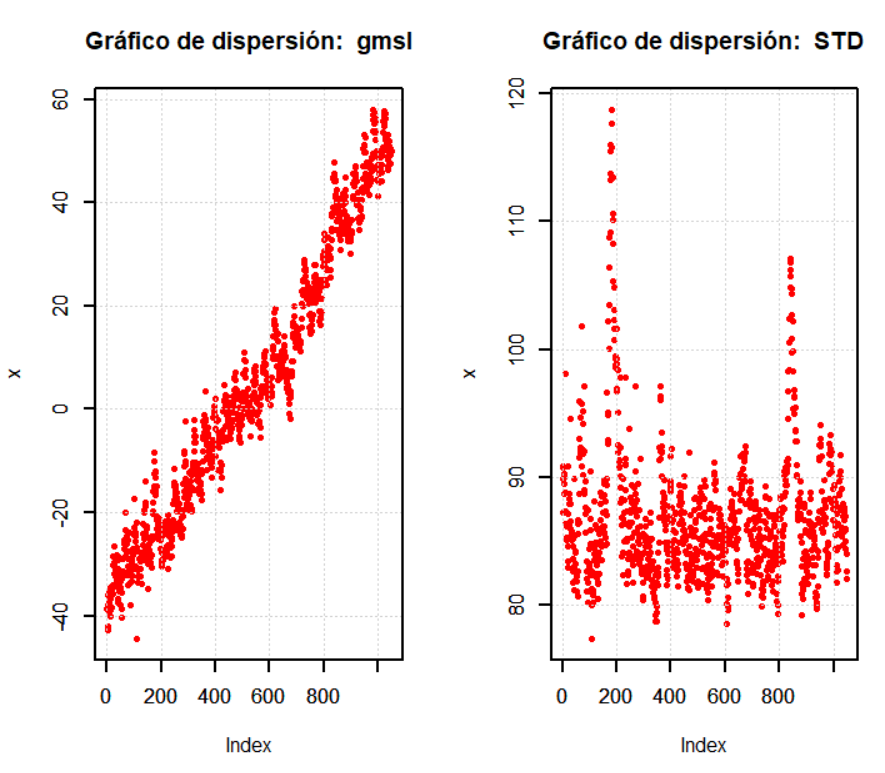
\includegraphics[scale = 0.4]{GraphDisp1.png}
    \caption{Gráficas de dispersión: A su izquierda, se presenta la gráfica de dispersión de \(GMSL\), mientras que, a su derecha puede ver la gráfica de dispersión de \(STD\).}
    \label{fig:1}
\end{figure}

\subsection{Bondad y ajuste GMSL y STD.}
\begin{figure}[htb]
    \centering
    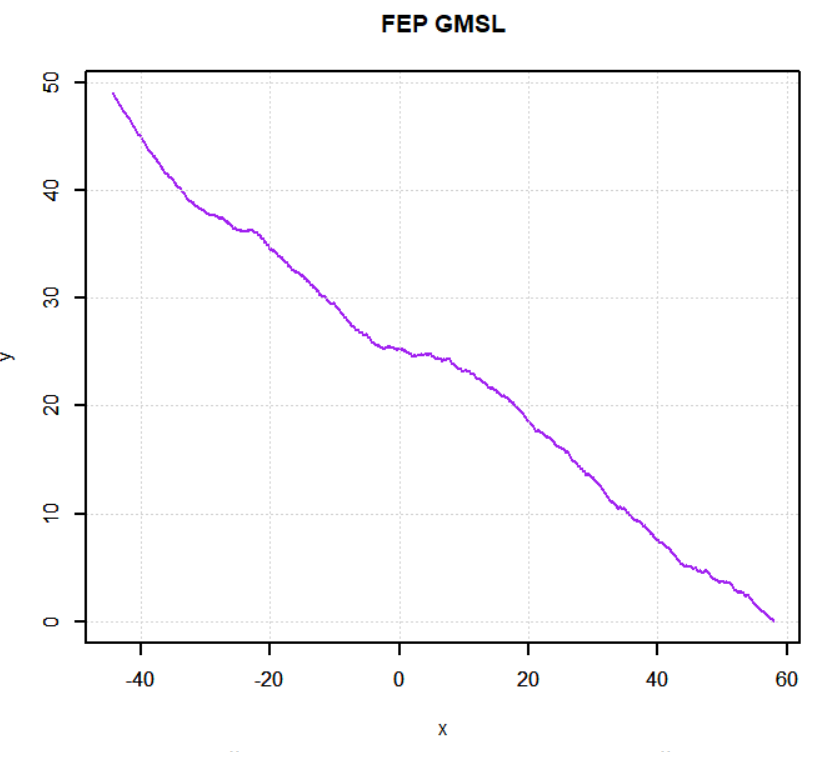
\includegraphics[scale = 0.4]{Incisob/FepGMSL.png}
    \caption{Gráfica Fep Empírica para las observaciones de GMSL. }
    \label{fig:2}
\end{figure}

\begin{figure}[htb]
    \centering
    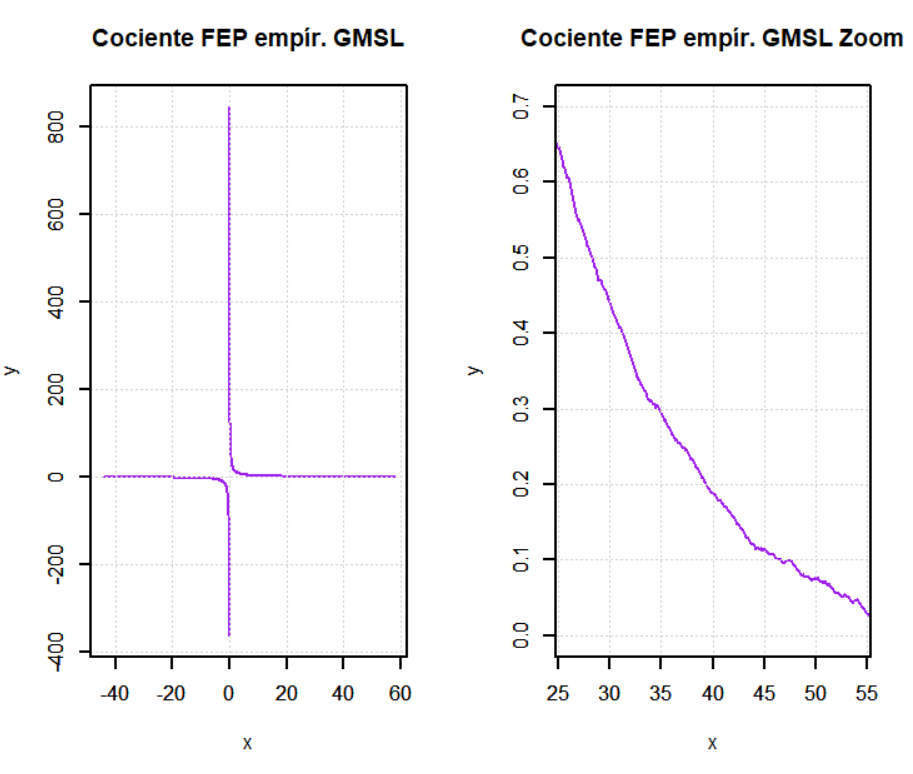
\includegraphics[scale = 0.4]{Incisob/CocFepGmls.png}
    \caption{Gráfica Cociente Fep Empírico para las observaciones de GMSL. }
    \label{fig:3}
\end{figure}

\begin{figure}[htb]
    \centering
    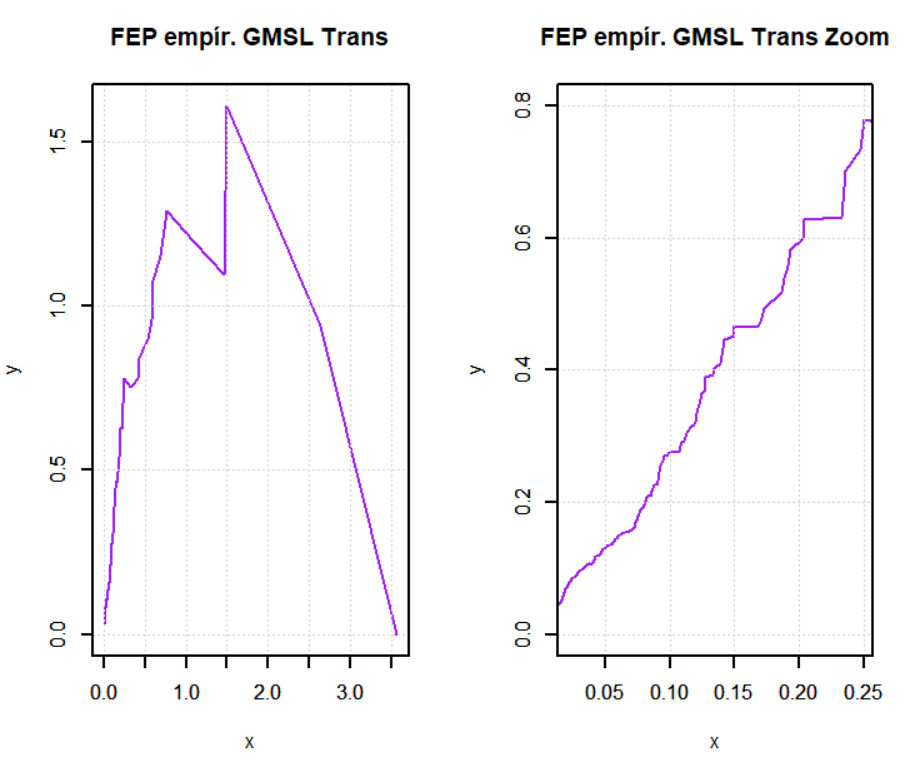
\includegraphics[scale = 0.4]{Incisob/FepGMLSTrans.png}
    \caption{Gráfica Fep Empírica para las observaciones de GMSL transformadas. }
    \label{fig:4}
\end{figure}

\begin{figure}[htb]
    \centering
    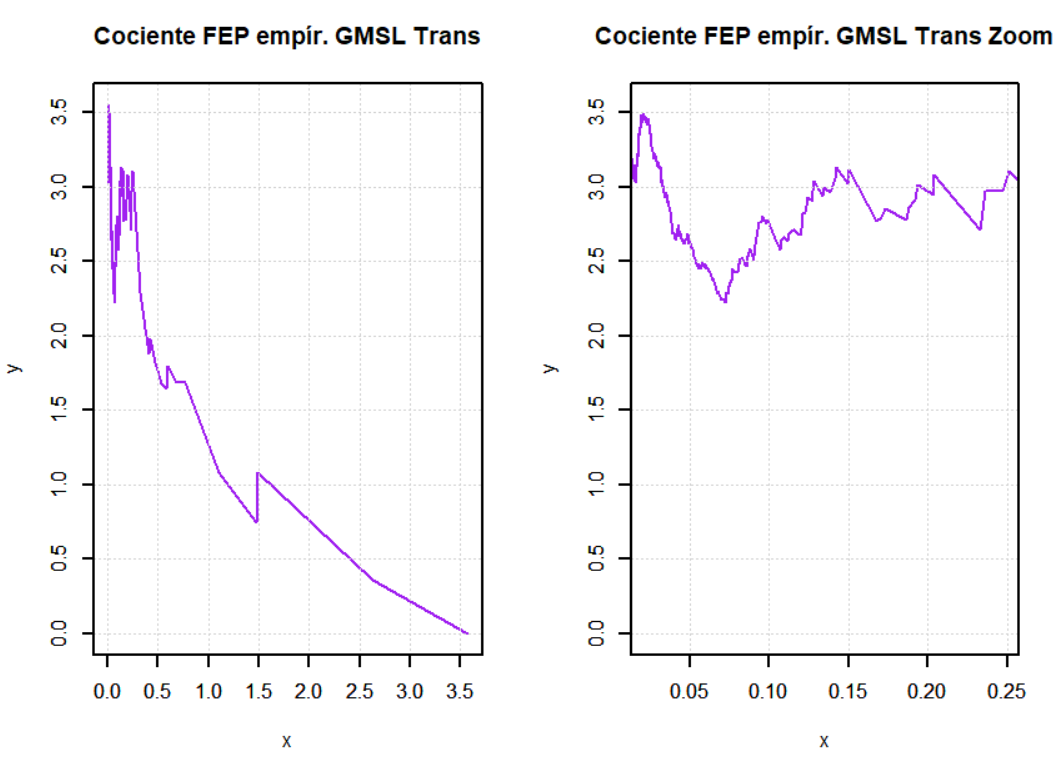
\includegraphics[scale = 0.4]{Incisob/CocFepGMLSTrans.png}
    \caption{Gráfica Cociente Fep Empírico para las observaciones de GMSL transformadas. }
    \label{fig:5}
\end{figure}

\begin{figure}[htb]
    \centering
    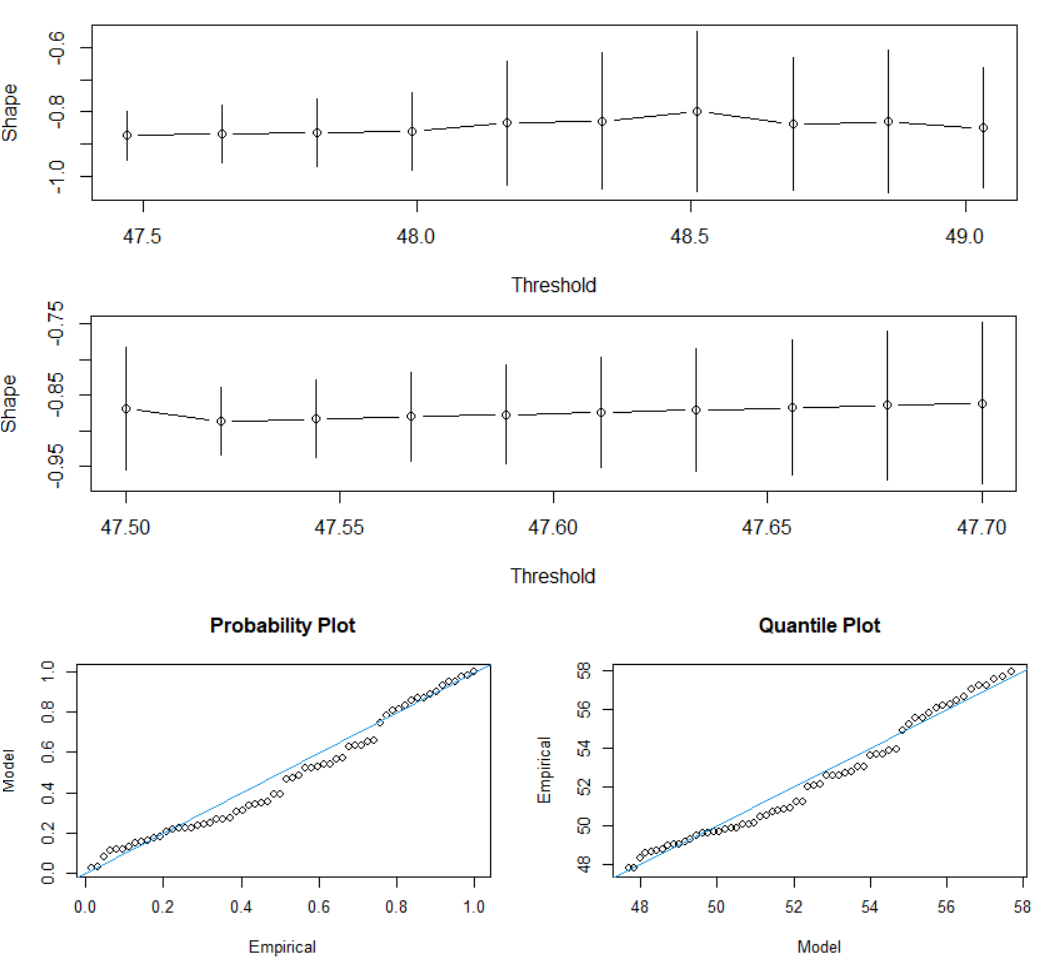
\includegraphics[scale = 0.4]{Incisob/AP1.png}
    \caption{Gráficas de selección de umbral y bondad de ajuste de una GPD\((\xi_1,a(u_1))\) a los datos en GMSL. Umbral seleccionado: \(u_1 = 47.55\). Estimaciones máximo verosímiles: \(a_1 =a(u_1) = 9.182\) y \(\xi_1 =  -0.883\).}
    \label{fig:6}
\end{figure}

\begin{figure}[htb]
    \centering
    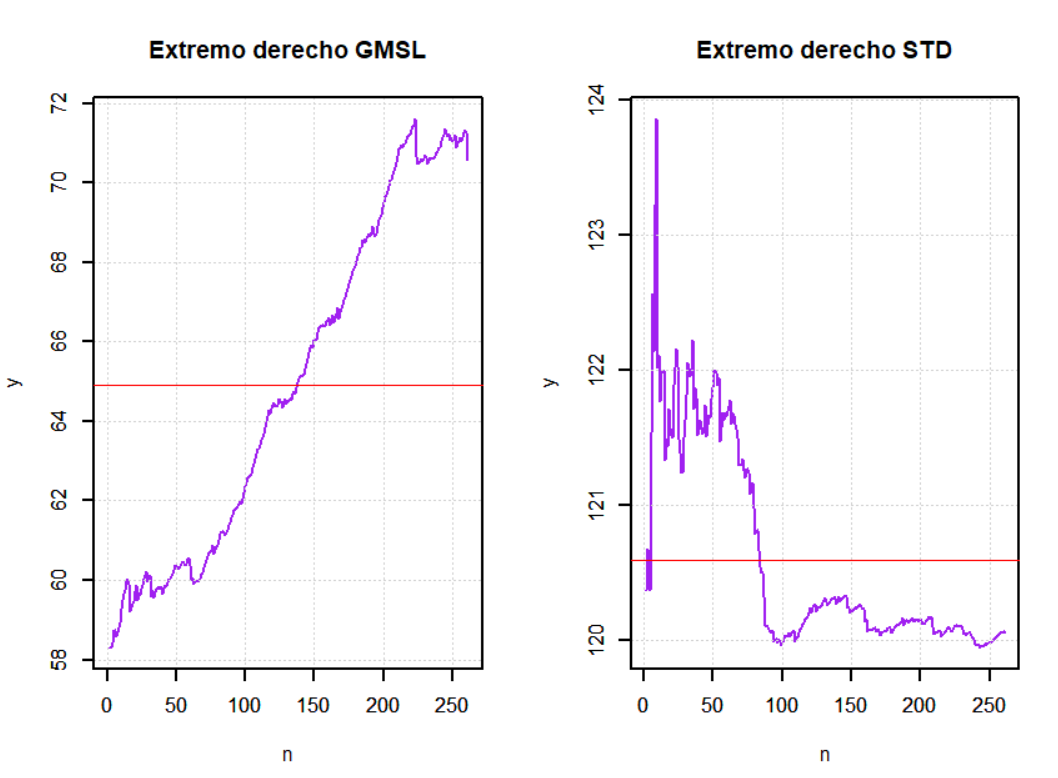
\includegraphics[scale = 0.5]{Incisob/EXTREMOSDERES.png}
    \caption{Estimación extremos derechos: Para ambas distribuciones mediante la metodología vista en ayudantía. Malla de valores para \(k_{n} \in \kis{1, \hdots, \floor{n^{0.8}}}\) y \(n = 1048\).}
    \label{fig:6.1}
\end{figure}


\begin{figure}[htb]
    \centering
    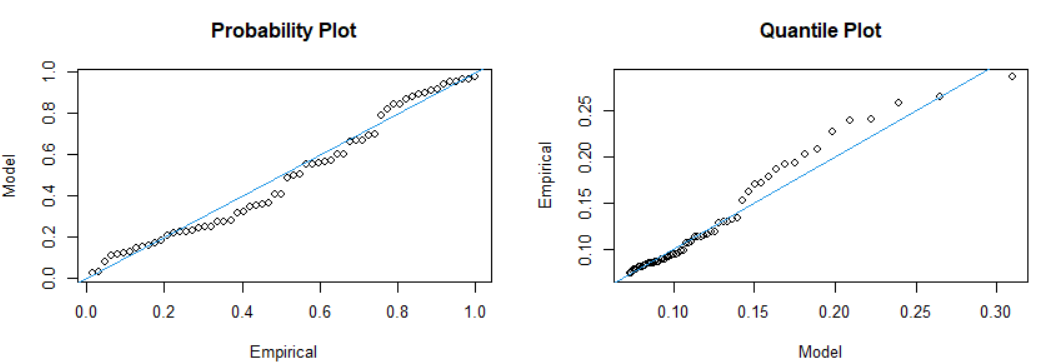
\includegraphics[scale = 0.4]{Incisob/AP1trans.png}
    \caption{Gráficas de bondad de ajuste GPD a datos transformados: Ajuste de una GPD\((\xi,a(u'))\) a los datos transformados de \(GMSL\) con: \(u' = 0.072\), \(\xi = 0.071\) y \(a(u') = 0.049\).}
    \label{fig:7}   
\end{figure}

\begin{figure}[htb]
    \centering
    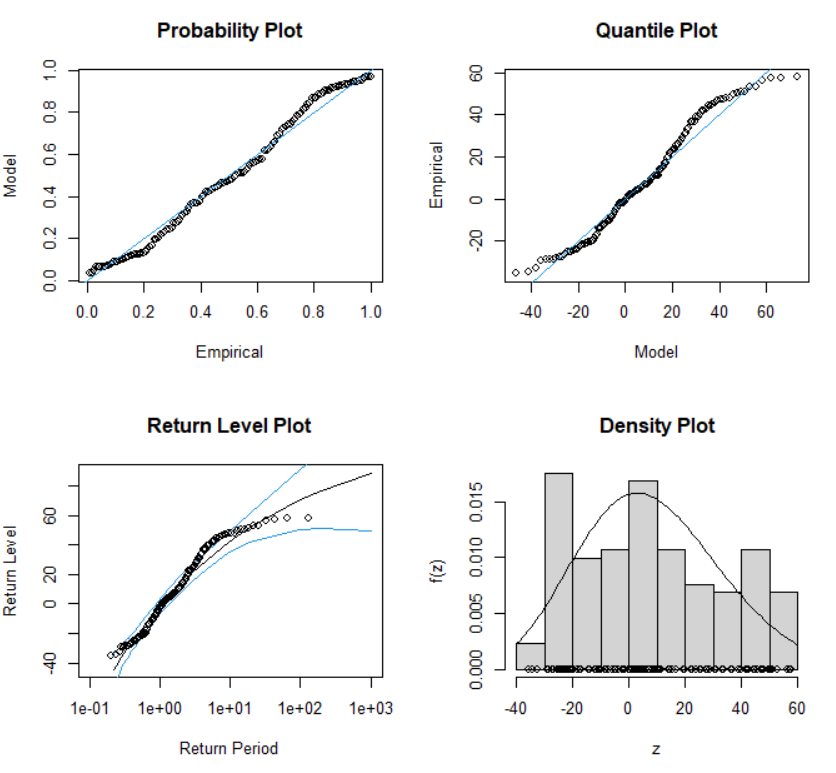
\includegraphics[scale = 0.4]{Incisob/gevfitgmsl.png}
    \caption{Gráficas de bondad de ajuste DGVE a datos de máximos: Ajuste de una DGVE\((\xi,a,b)\) a los datos de máximos por año de \(GMSL\) con parámetros: \(localización=b = 5.155\), \(escala =a = 23.791\) y \(forma = \xi'= -0.222\).}
    \label{fig:7.1}   
\end{figure}


\begin{figure}[htb]
    \centering
    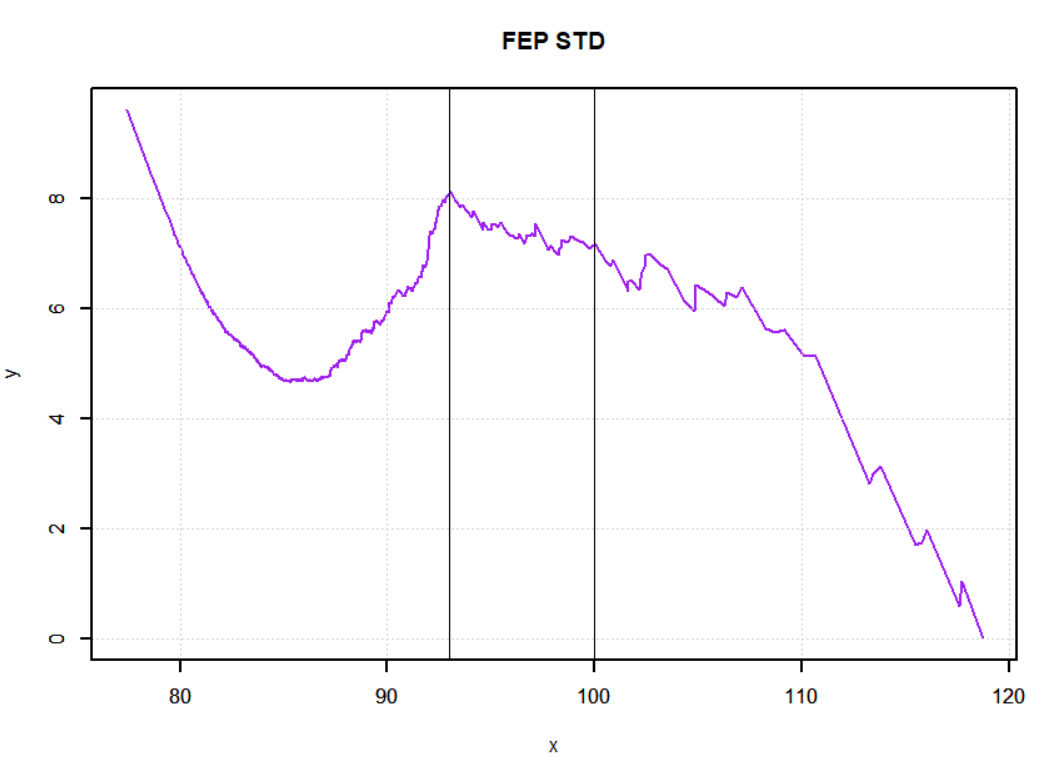
\includegraphics[scale = 0.4]{Incisob/FepSTD.png}
    \caption{Gráfica Fep Empírica para las observaciones de \(STD\). }
    \label{fig:8}
\end{figure}

\begin{figure}[htb]
    \centering
    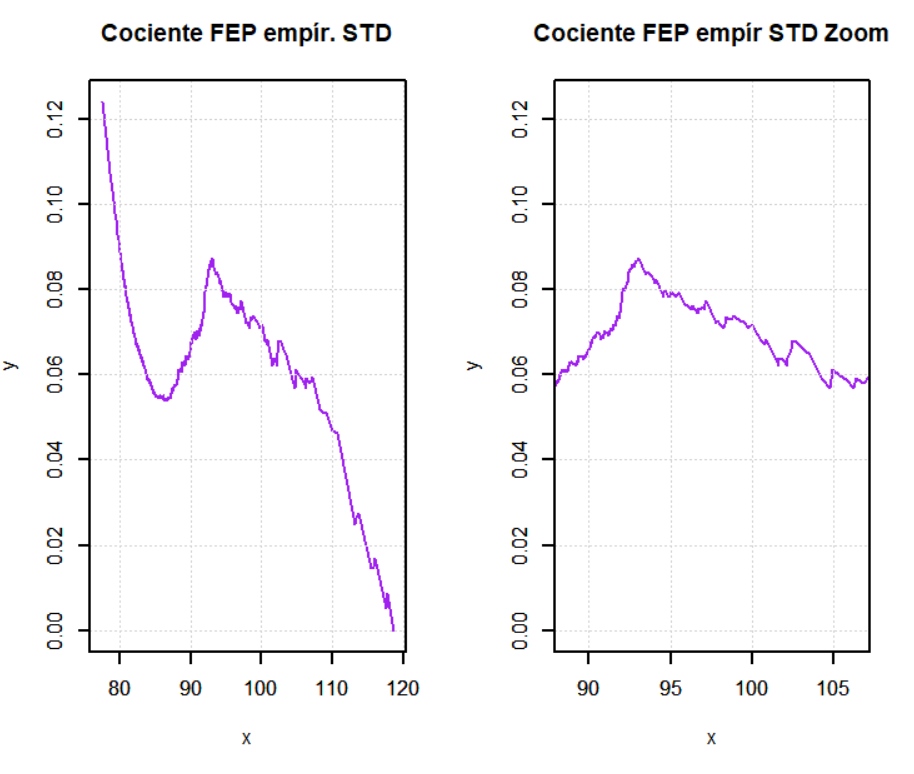
\includegraphics[scale = 0.4]{Incisob/CocFepSTD.png}
    \caption{Gráfica Cociente Fep Empírico para las observaciones de \(STD\).}
    \label{fig:9}
\end{figure}

\begin{figure}[htb]
    \centering
    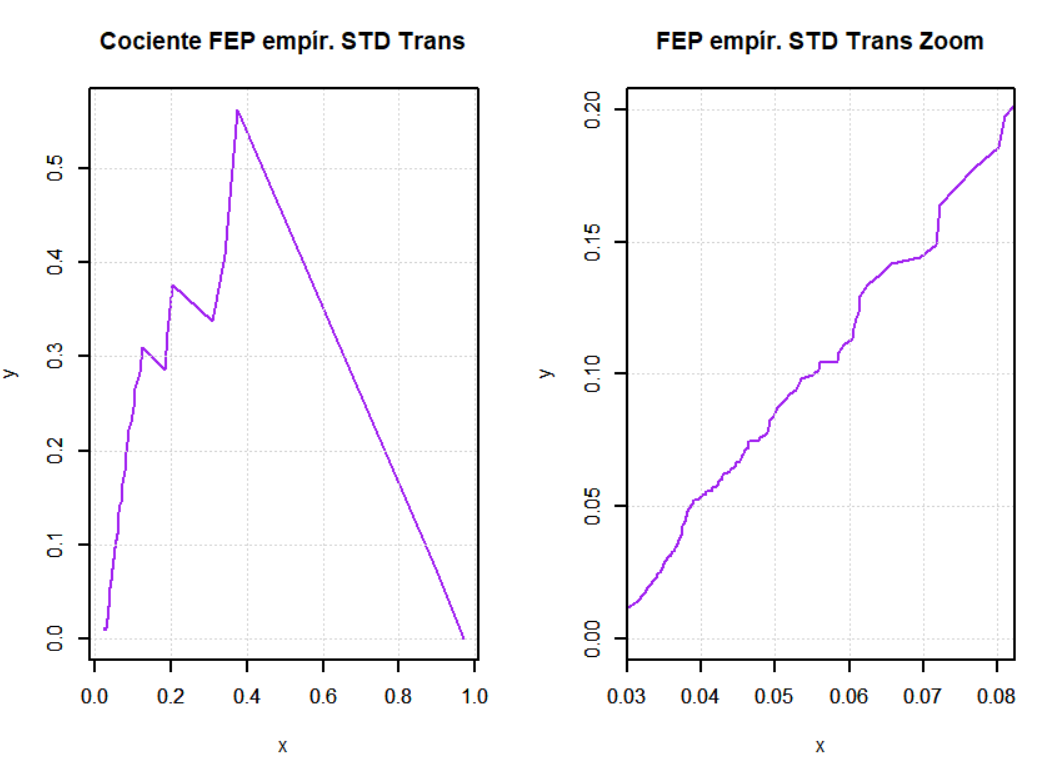
\includegraphics[scale = 0.4]{Incisob/FepSTDTrans.png}
    \caption{Gráfica Fep Empírica para las observaciones de \(STD\) transformadas. }
    \label{fig:10}
\end{figure}

\begin{figure}[htb]
    \centering
    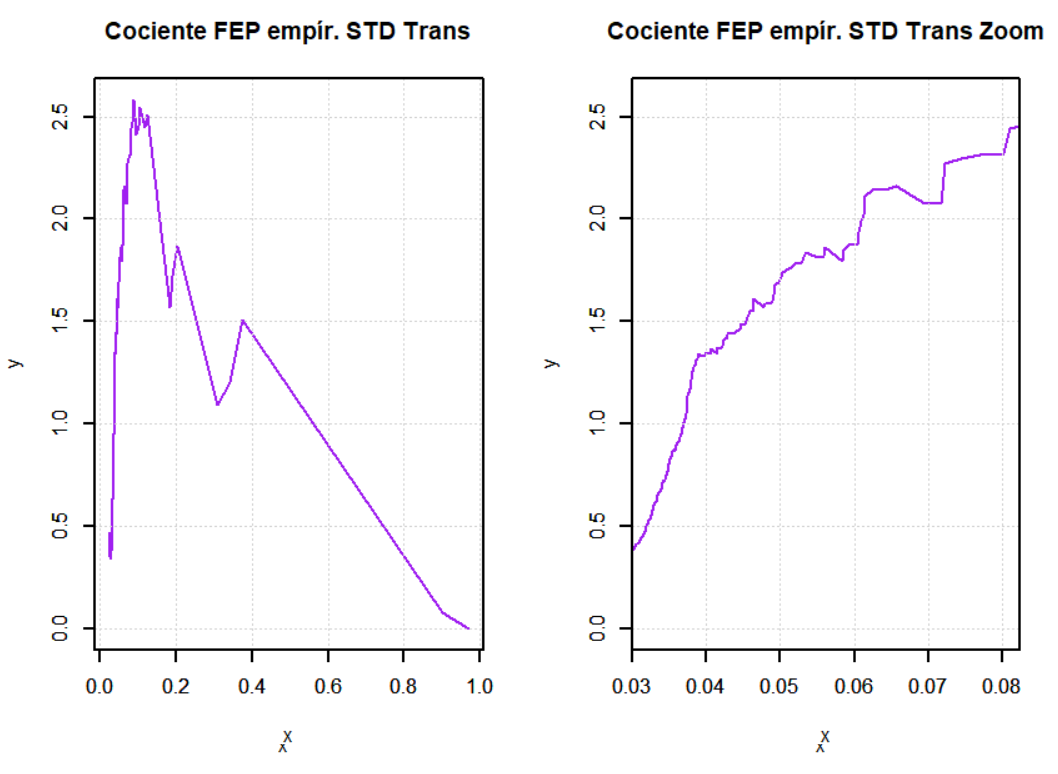
\includegraphics[scale = 0.4]{Incisob/CocFepSTDTrans.png}
    \caption{Gráfica Cociente Fep Empírico para las observaciones de \(STD\) transformadas. }
    \label{fig:11}
\end{figure}

\begin{figure}[htb]
    \centering
    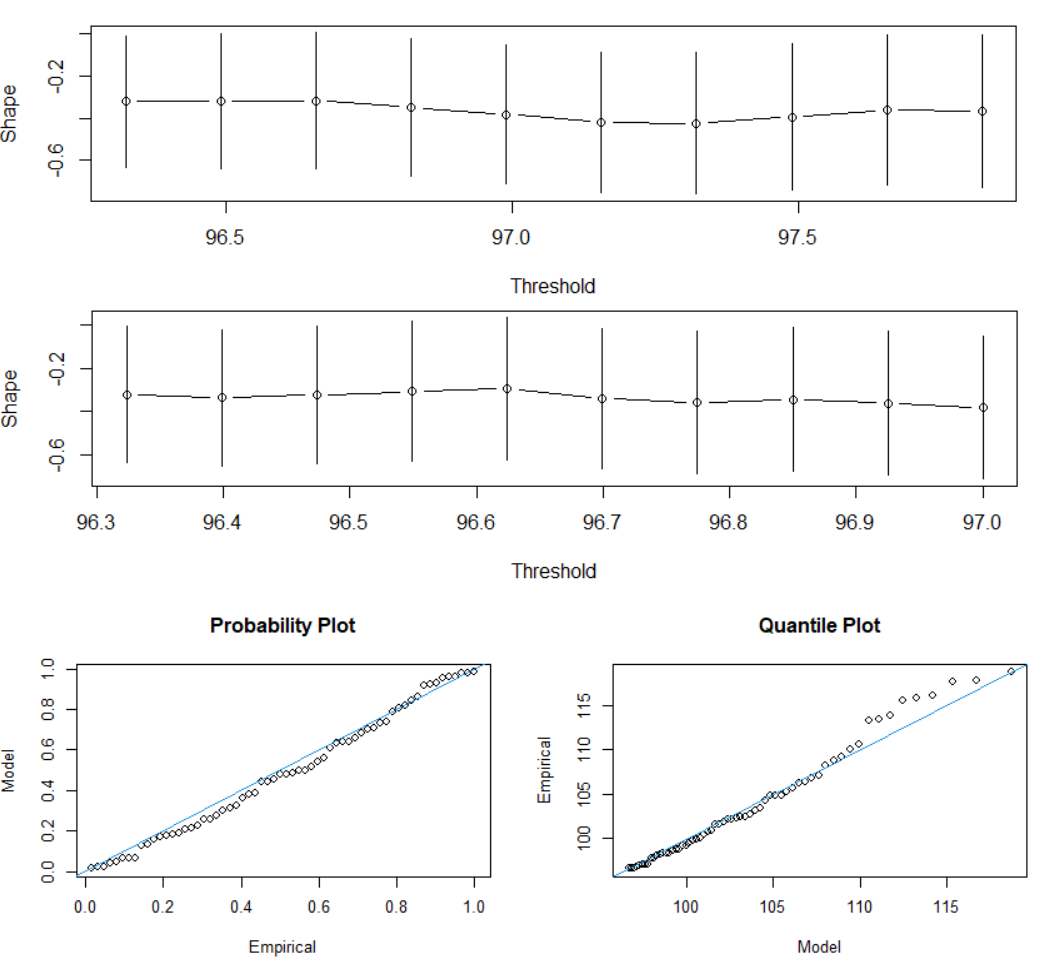
\includegraphics[scale = 0.4]{Incisob/AP2.png}
    \caption{Gráficas de selección de umbral y bondad de ajuste de una GPD\((\xi_2,a(u_2))\) a los datos en \(STD\). Umbral seleccionado: \(u_2 = 96.5\). Estimaciones máximo verosímiles: \(a_2 =a(u_2) = 9.657 \) y \(\xi_2 =-0.318\).}
    \label{fig:12}
\end{figure}

\begin{figure}[htb]
    \centering
    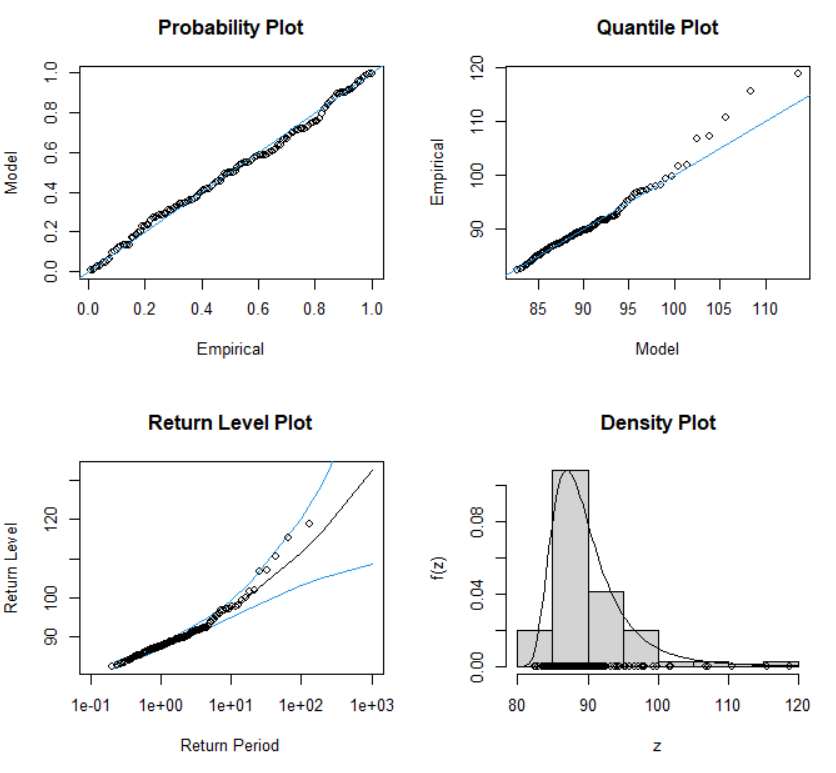
\includegraphics[scale = 0.4]{Incisob/gevfitSTD.png}
    \caption{Gráficas de bondad de ajuste DGVE a datos de máximos: Ajuste de una DGVE\((\xi,a,b)\) a los datos de máximos por año de \(STD\) con parámetros: \(localización=b = 90.433\), \(escala =a = 3.194\) y \(forma = \xi'=  0.547\).}
    \label{fig:14.1}   
\end{figure}     


\begin{figure}[htb]
    \centering
    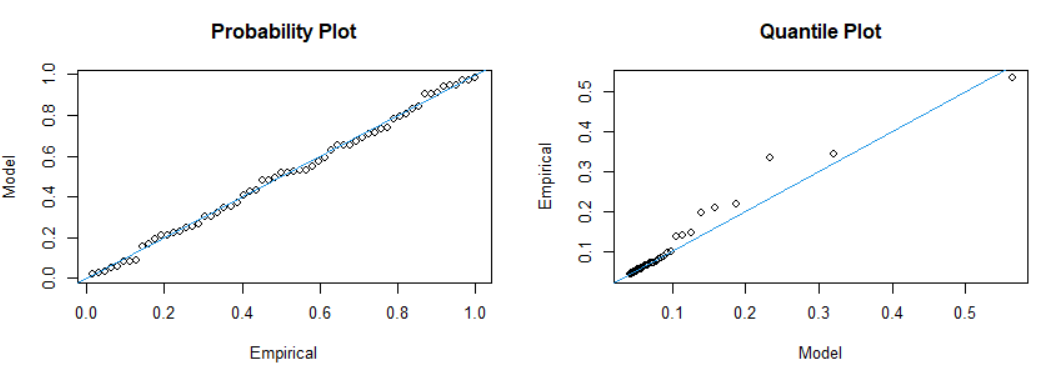
\includegraphics[scale = 0.4]{Incisob/AP2trans.png}
    \caption{Gráficas de bondad de ajuste GPD a datos transformados: Ajuste de una GPD\((\xi,a(u))\) a los datos transformados de \(STD\) con: \(u = 0.072\), \(\xi = 0.871\) y \(a(u) = 0.013\).}
    \label{fig:14}   
\end{figure}

\begin{figure}[htb]
    \centering
    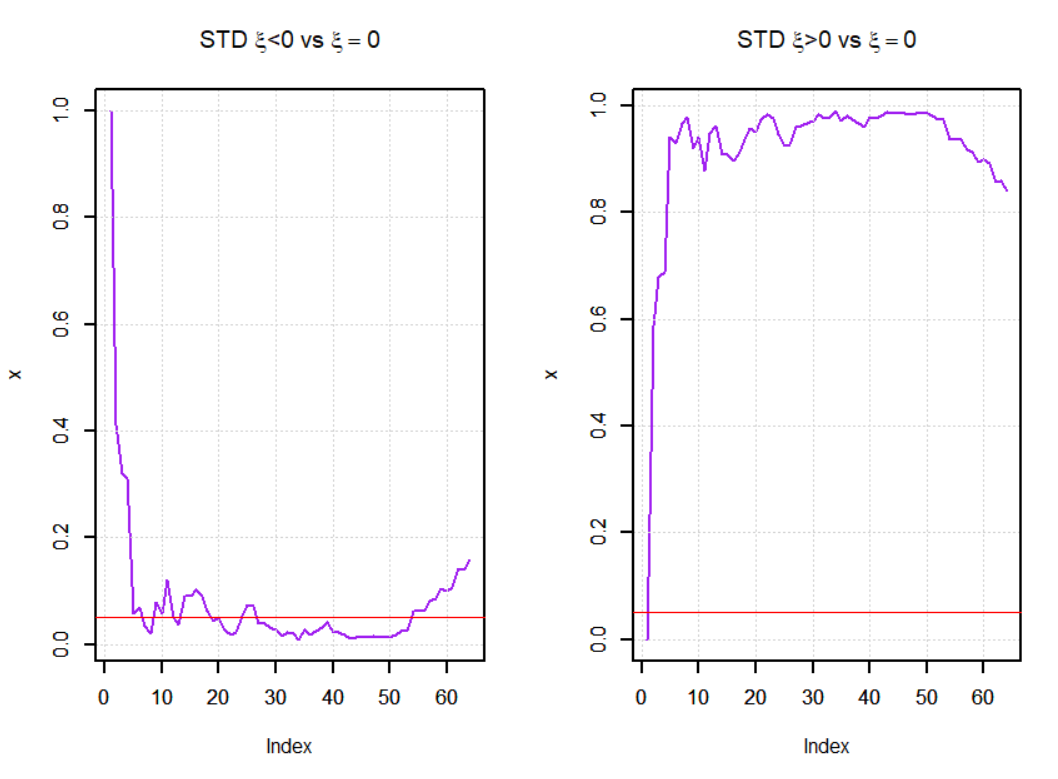
\includegraphics[scale = 0.4]{Incisob/PH1.png}
    \caption{Pruebas de hipótesis para los datos \(STD\) con estadística \(G_{n,k}(0)\). A su izquierda, gráfica del contraste \(\mathcal{H}_0: \xi = 0\) vs \(\mathcal{H}_1: \xi < 0\). A su derecha, gráfica del contraste \(\mathcal{H}_0: \xi = 0\) vs \(\mathcal{H}_1: \xi > 0\). Malla de valores \(k_{n}\in\kis{1, \hdots, \floor{n^{0.6}}}\), \(n = 1048\).}
    \label{fig:15}
\end{figure}
\subsection{Bondad y ajuste diffGMSL.}

\begin{figure}[htb]
    \centering
    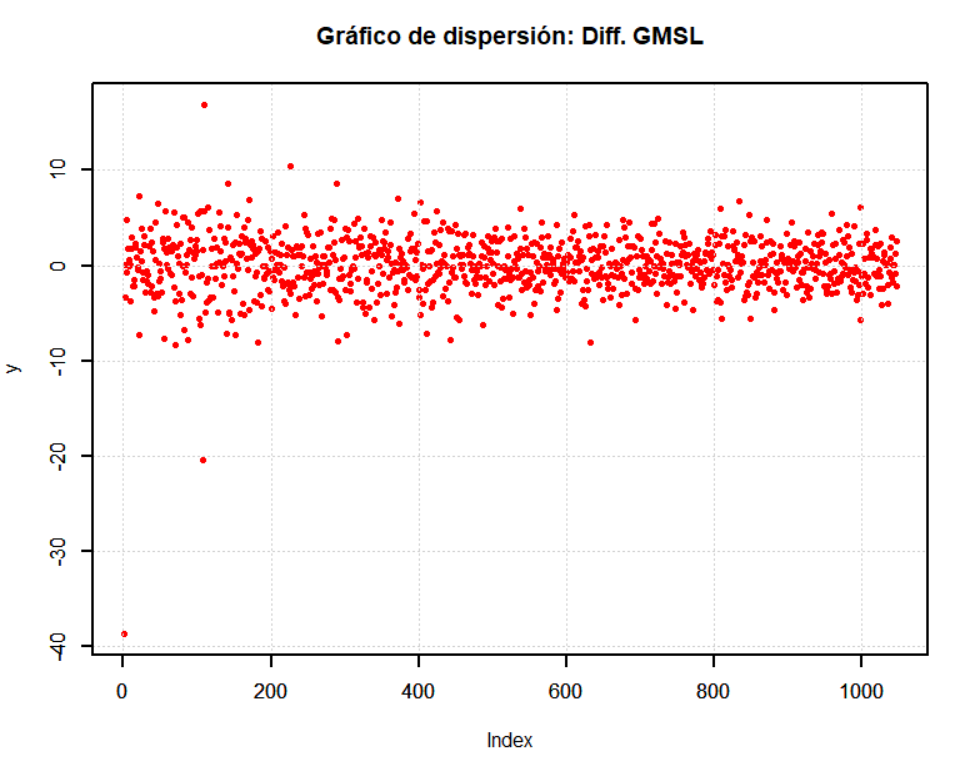
\includegraphics[scale = 0.4]{incisoc/DDisp.png}
    \caption{Gráfica de dispersión para los datos de diferencias \(GMSL\).}
    \label{fig:17}
\end{figure}


\begin{figure}[htb]
    \centering
    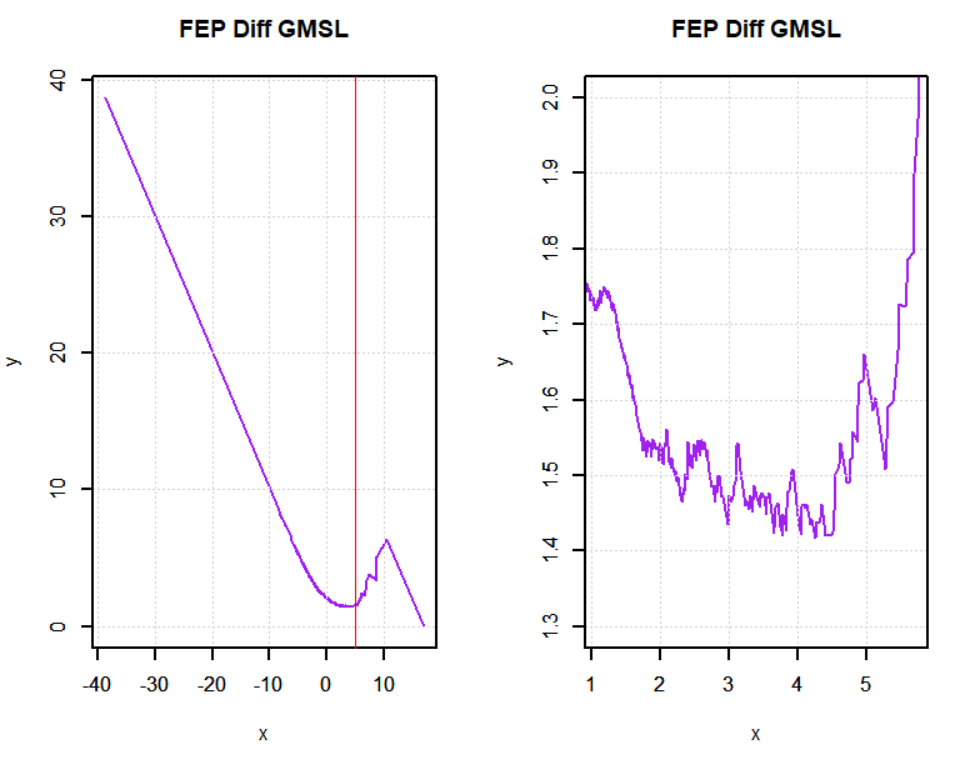
\includegraphics[scale = 0.4]{incisoc/DFepGMSL.png}
    \caption{Gráfica Fep Empírica para los datos de diferencias \(GMSL\).}
    \label{fig:17.1}
\end{figure}

\begin{figure}[htb]
    \centering
    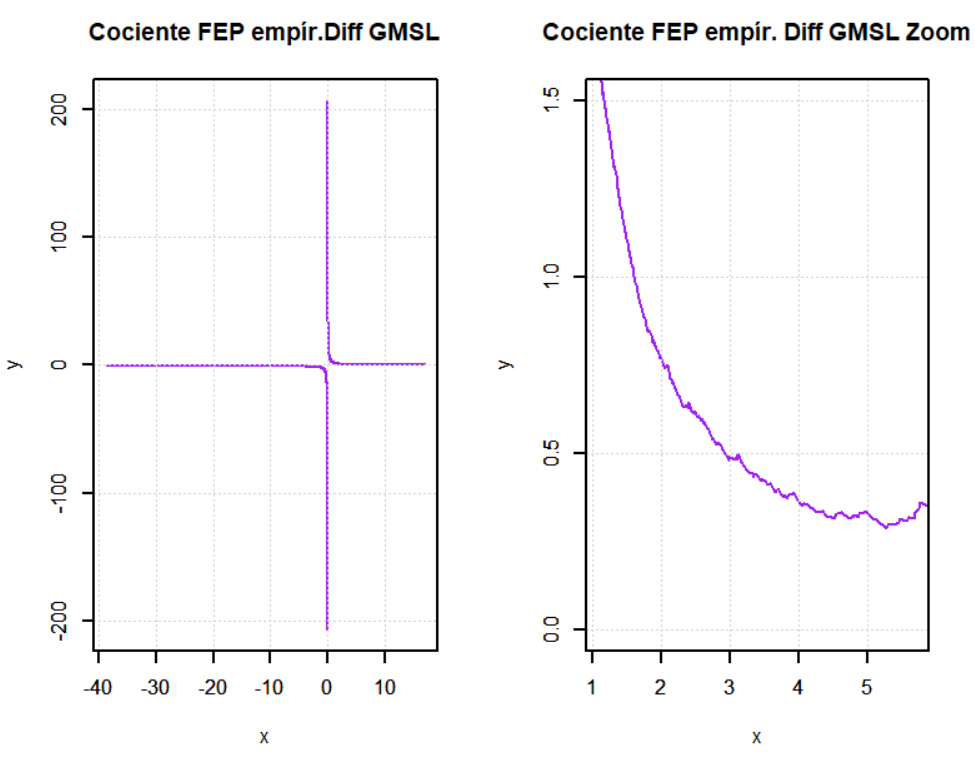
\includegraphics[scale = 0.4]{incisoc/DCocFepGMSL.png}
    \caption{Gráfica Cociente Fep Empírico para los datos de diferencias de \(GMSL\).}
    \label{fig:18}
\end{figure}

\begin{figure}[htb]
    \centering
    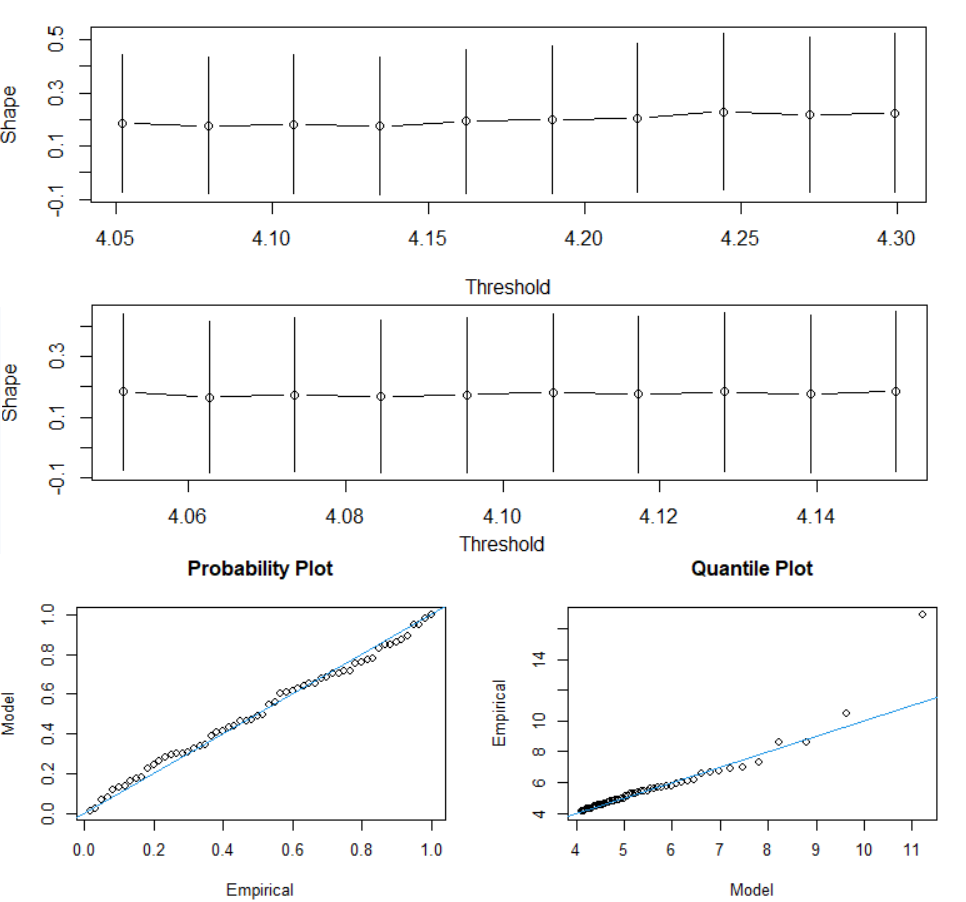
\includegraphics[scale = 0.4]{incisoc/DAp1GMSL.png}
    \caption{Gráficas de selección de umbral y bondad de ajuste de una GPD\((\xi_3,a(u_3))\) a los datos de diferencias de \(GMSL\). Umbral seleccionado: \(u_3 = 4.10\). Estimaciones máximo verosímiles:  \(a_3 =a(u_3) = 1.178\) y \(\xi_3 = 0.177\).}
    \label{fig:19}
\end{figure}

\begin{comment}
\begin{figure}[htb]
    \centering
    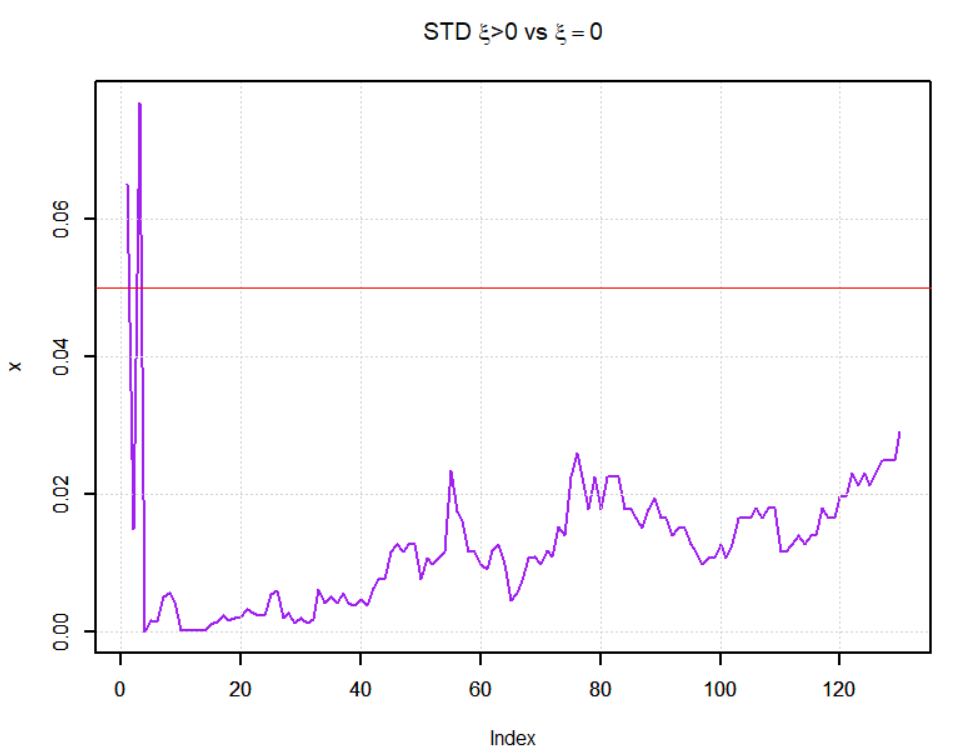
\includegraphics[scale = 0.4]{incisoc/DPh1.png}
    \caption{Prueba de hipótesis para los datos de diferencias \(GMSL\) con estadística \(G_{n,k}(0)\). Gráfica del contraste \(\mathcal{H}_0: \xi = 0\) vs \(\mathcal{H}_1: \xi > 0\). Malla de valores \(k_{n}\in\kis{1, \hdots, \floor{n^{0.7}}}.\), \(n = 1048\).}
    \label{fig:20}
\end{figure}
\end{comment}
\subsection{Bondad y ajuste diffSTD.}

\begin{figure}[htb]
    \centering
    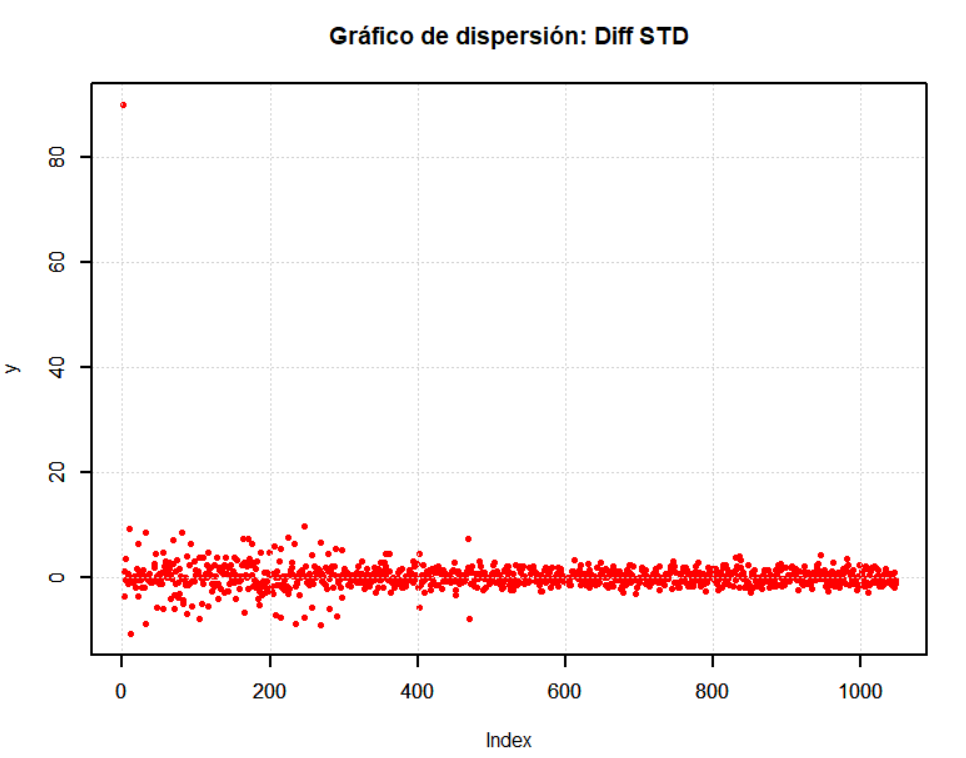
\includegraphics[scale = 0.4]{incisoc/DSDisp.png}
    \caption{Gráfica de dispersión para los datos de diferencias \(STD\).}
    \label{fig:21}
\end{figure}

\begin{figure}[htb]
    \centering
    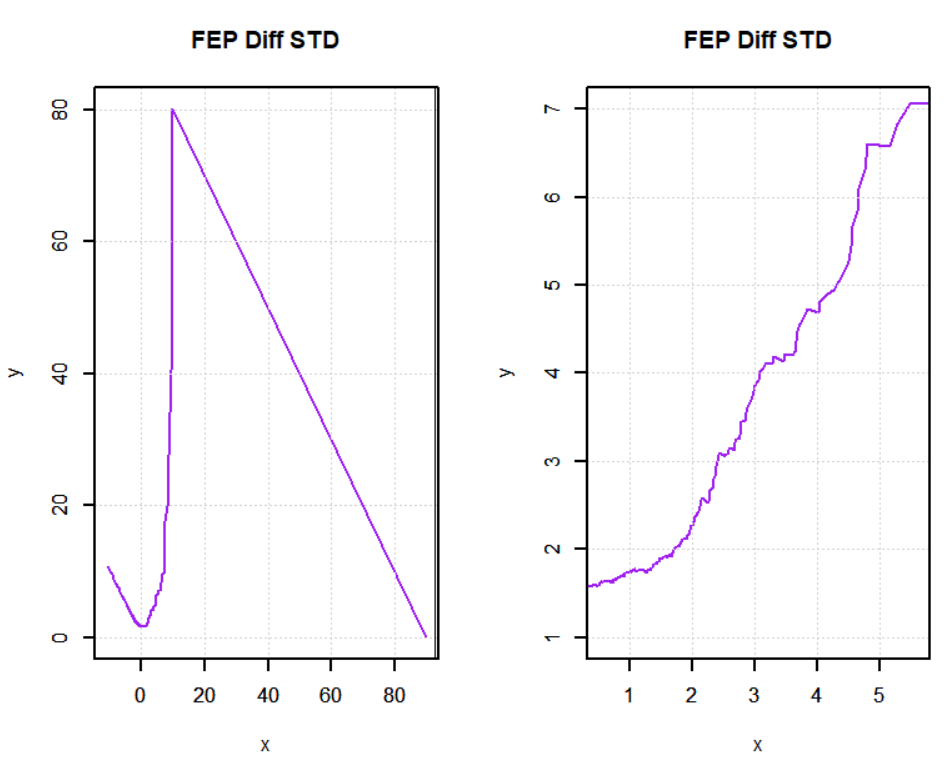
\includegraphics[scale = 0.4]{incisoc/DFepSTD.png}
    \caption{Gráfica Fep Empírica para los datos de diferencias \(STD\).}
    \label{fig:22}
\end{figure}

\begin{figure}[htb]
    \centering
    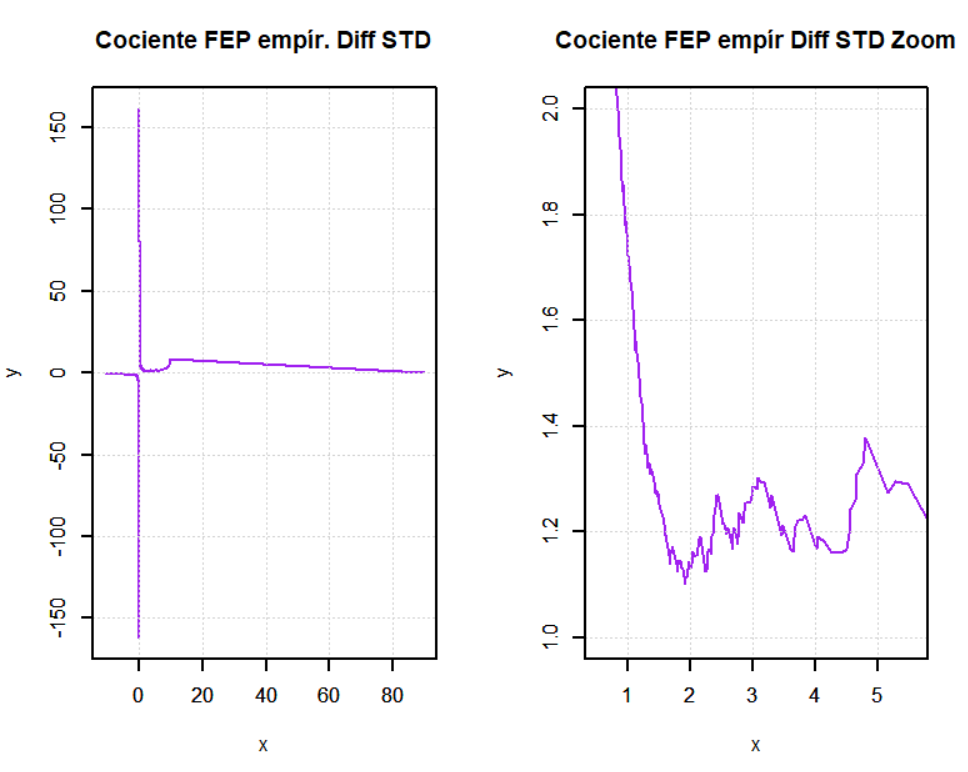
\includegraphics[scale = 0.4]{incisoc/DCocFepSTD.png}
    \caption{Gráfica Cociente Fep Empírico para las observaciones de diferencias de \(STD\).}
    \label{fig:23}
\end{figure}

\begin{figure}[htb]
    \centering
    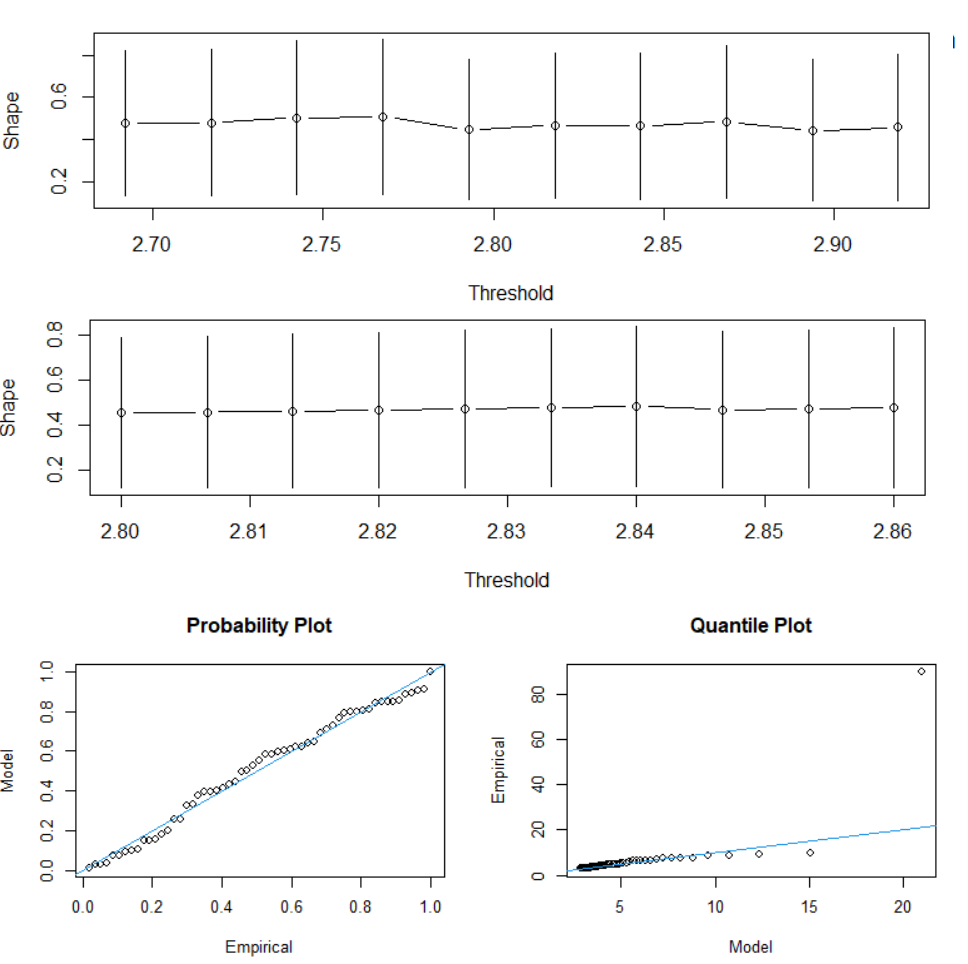
\includegraphics[scale = 0.4]{incisoc/DAp1STD.png}
    \caption{Gráficas de selección de umbral y bondad de ajuste de una GPD\((\xi_4,a(u_4))\) a los datos de diferencias de \(STD\). Umbral seleccionado: \(u_4 = 2.83\). Estimaciones máximo verosímiles: \(a_4 =a(u_4) = 0.315\) y \(\xi_4 =  0.180\).}
    \label{fig:24} 
\end{figure}
\section{Gráficas para diferencias Máximas.}
\begin{figure}[htb]
    \centering
    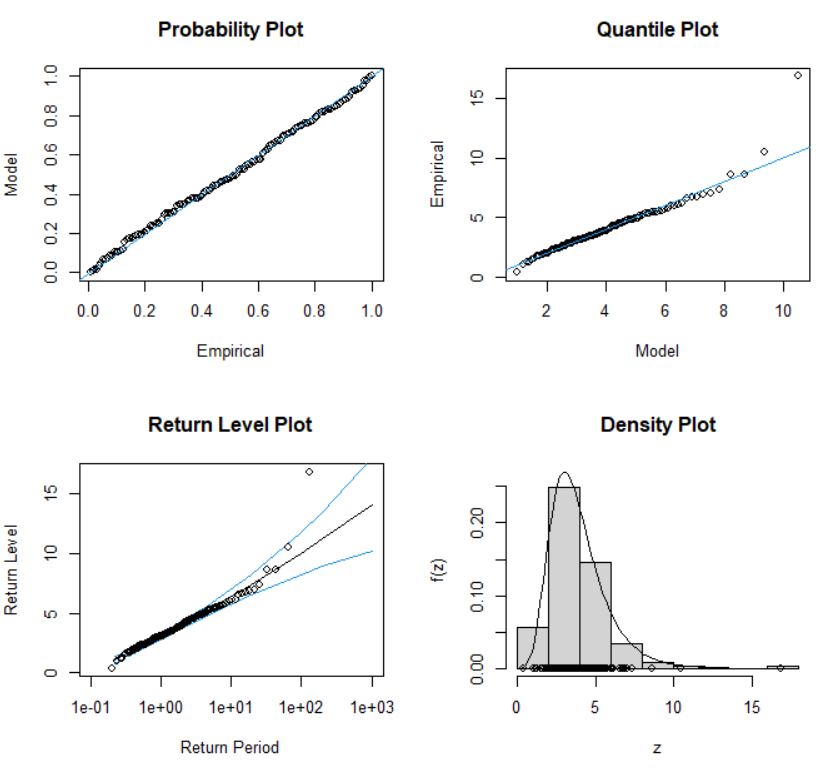
\includegraphics[scale = 0.4]{incisoc/DGVEaj.png}
    \caption{Gráficas de bondad de ajuste DGVE a datos de máximos: Ajuste de una DGVE\((\xi',a,b)\) a los datos de máximos  de \(diffGMSL\) con parámetros: \(localización=b = 3.070\), \(escala =a =  1.362 \) y \(forma = \xi'= 0.046\).}
    \label{fig:14.11}   
\end{figure}    

\begin{figure}[htb]
    \centering
    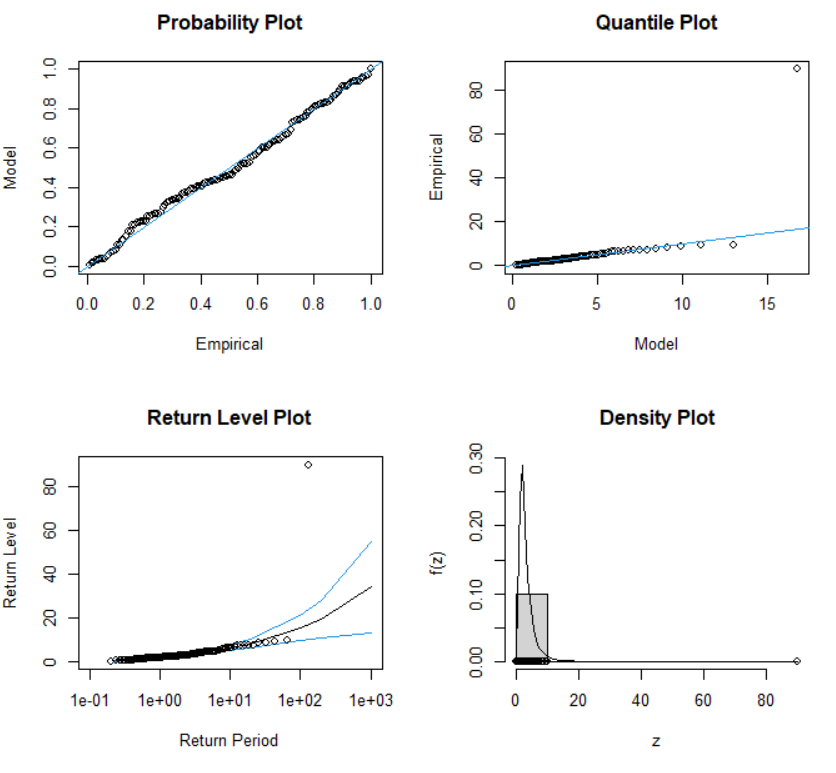
\includegraphics[scale = 0.4]{incisoc/DGVEajS.png}
    \caption{Gráficas de bondad de ajuste DGVE de máximos: Ajuste de una DGVE\((\xi',a,b)\) a los datos de máximos \(diffSTD\) con parámetros: \(localización=b = 1.828\), \(escala =a = 1.272\) y \(forma = \xi'=  0.320\).}
    \label{fig:14.12}    
\end{figure}        



\end{document}
